\documentclass[twoside]{book}

% Packages required by doxygen
\usepackage{fixltx2e}
\usepackage{calc}
\usepackage{doxygen}
\usepackage[export]{adjustbox} % also loads graphicx
\usepackage{graphicx}
\usepackage[utf8]{inputenc}
\usepackage{makeidx}
\usepackage{multicol}
\usepackage{multirow}
\PassOptionsToPackage{warn}{textcomp}
\usepackage{textcomp}
\usepackage[nointegrals]{wasysym}
\usepackage[table]{xcolor}

% Font selection
\usepackage[T1]{fontenc}
\usepackage[scaled=.90]{helvet}
\usepackage{courier}
\usepackage{amssymb}
\usepackage{sectsty}
\renewcommand{\familydefault}{\sfdefault}
\allsectionsfont{%
  \fontseries{bc}\selectfont%
  \color{darkgray}%
}
\renewcommand{\DoxyLabelFont}{%
  \fontseries{bc}\selectfont%
  \color{darkgray}%
}
\newcommand{\+}{\discretionary{\mbox{\scriptsize$\hookleftarrow$}}{}{}}

% Page & text layout
\usepackage{geometry}
\geometry{%
  a4paper,%
  top=2.5cm,%
  bottom=2.5cm,%
  left=2.5cm,%
  right=2.5cm%
}
\tolerance=750
\hfuzz=15pt
\hbadness=750
\setlength{\emergencystretch}{15pt}
\setlength{\parindent}{0cm}
\setlength{\parskip}{3ex plus 2ex minus 2ex}
\makeatletter
\renewcommand{\paragraph}{%
  \@startsection{paragraph}{4}{0ex}{-1.0ex}{1.0ex}{%
    \normalfont\normalsize\bfseries\SS@parafont%
  }%
}
\renewcommand{\subparagraph}{%
  \@startsection{subparagraph}{5}{0ex}{-1.0ex}{1.0ex}{%
    \normalfont\normalsize\bfseries\SS@subparafont%
  }%
}
\makeatother

% Headers & footers
\usepackage{fancyhdr}
\pagestyle{fancyplain}
\fancyhead[LE]{\fancyplain{}{\bfseries\thepage}}
\fancyhead[CE]{\fancyplain{}{}}
\fancyhead[RE]{\fancyplain{}{\bfseries\leftmark}}
\fancyhead[LO]{\fancyplain{}{\bfseries\rightmark}}
\fancyhead[CO]{\fancyplain{}{}}
\fancyhead[RO]{\fancyplain{}{\bfseries\thepage}}
\fancyfoot[LE]{\fancyplain{}{}}
\fancyfoot[CE]{\fancyplain{}{}}
\fancyfoot[RE]{\fancyplain{}{\bfseries\scriptsize Generated by Doxygen }}
\fancyfoot[LO]{\fancyplain{}{\bfseries\scriptsize Generated by Doxygen }}
\fancyfoot[CO]{\fancyplain{}{}}
\fancyfoot[RO]{\fancyplain{}{}}
\renewcommand{\footrulewidth}{0.4pt}
\renewcommand{\chaptermark}[1]{%
  \markboth{#1}{}%
}
\renewcommand{\sectionmark}[1]{%
  \markright{\thesection\ #1}%
}

% Indices & bibliography
\usepackage{natbib}
\usepackage[titles]{tocloft}
\setcounter{tocdepth}{3}
\setcounter{secnumdepth}{5}
\makeindex

% Hyperlinks (required, but should be loaded last)
\usepackage{ifpdf}
\ifpdf
  \usepackage[pdftex,pagebackref=true]{hyperref}
\else
  \usepackage[ps2pdf,pagebackref=true]{hyperref}
\fi
\hypersetup{%
  colorlinks=true,%
  linkcolor=blue,%
  citecolor=blue,%
  unicode%
}

% Custom commands
\newcommand{\clearemptydoublepage}{%
  \newpage{\pagestyle{empty}\cleardoublepage}%
}

\usepackage{caption}
\captionsetup{labelsep=space,justification=centering,font={bf},singlelinecheck=off,skip=4pt,position=top}

%===== C O N T E N T S =====

\begin{document}

% Titlepage & ToC
\hypersetup{pageanchor=false,
             bookmarksnumbered=true,
             pdfencoding=unicode
            }
\pagenumbering{alph}
\begin{titlepage}
\vspace*{7cm}
\begin{center}%
{\Large sc\+:\+:list \\[1ex]\large 1 }\\
\vspace*{1cm}
{\large Generated by Doxygen 1.8.14}\\
\end{center}
\end{titlepage}
\clearemptydoublepage
\pagenumbering{roman}
\tableofcontents
\clearemptydoublepage
\pagenumbering{arabic}
\hypersetup{pageanchor=true}

%--- Begin generated contents ---
\chapter{Introduction}
\label{md_README}
\Hypertarget{md_README}
This project implements {\ttfamily \mbox{\hyperlink{classsc_1_1list}{sc\+::list}}}, a {\ttfamily std\+::list} custom implementation.

The project was implemeted in a Programming class at federal University of Rio Grande do Norte.

\section*{Supported Operations}

The supported opperations are listed below.

\section*{Commom operations}


\begin{DoxyItemize}
\item {\ttfamily size\+\_\+type size() const} \+: return the number of elements in the container.
\item {\ttfamily void clear()} \+: remove (either logically or physically) all elements from the container.
\item {\ttfamily bool empty()} \+: returns true if the container contains no elements, and false otherwise.
\item {\ttfamily void push\+\_\+front( const T \& value )} \+: adds value to the front of the list.
\item {\ttfamily void push\+\_\+back( const T \& value )} \+: adds value to the end of the list.
\item {\ttfamily void pop\+\_\+back()} \+: removes the object at the end of the list.
\item {\ttfamily void pop\+\_\+front()} \+: removes the object at the front of the list.
\item {\ttfamily const T \& back() const} \+: returns the object at the end of the list.
\item {\ttfamily const T \& front() const} \+: returns the object at the beginning of the list.
\item {\ttfamily void assign( const T \& value )} \+: replaces the content of the list with copies of value {\ttfamily value} .
\end{DoxyItemize}

\section*{Operator overloading}


\begin{DoxyItemize}
\item {\ttfamily bool operator==( const vector\& lhs, const vector\& rhs )} \+: Checks if the contents of lhs and rhs are equal, that is, whether {\ttfamily lhs.\+size() == rhs.\+size()} and each element in lhs compares equal with the element in {\ttfamily rhs} at the same position.
\item {\ttfamily bool operator!=( const vector\& lhs, const vector\& rhs)} \+: Similar to the previous operator, but the opposite result.
\end{DoxyItemize}

\section*{Getting Iterator}


\begin{DoxyItemize}
\item {\ttfamily iterator begin()} \+: returns an {\ttfamily iterator} pointing to the first item in the list.
\item {\ttfamily const\+\_\+iterator cbegin() const} \+: returns a {\ttfamily constant iterator} pointing to the first item in the list.
\item {\ttfamily iterator end()} \+: returns an {\ttfamily iterator} pointing to the end mark in the list, i.\+e. the position just after the last element of the list.
\item {\ttfamily const\+\_\+iterator cend() const} \+: returns a {\ttfamily constant iterator} pointing to the end mark in the list, i.\+e. the position just after the last element of the list.
\end{DoxyItemize}

\section*{Iterator operations}


\begin{DoxyItemize}
\item {\ttfamily operator++()} \+: advances {\ttfamily iterator} to the next location within the list. We should provide both prefix and posfix form, or {\ttfamily ++it} and {\ttfamily it++} .
\item {\ttfamily operator$\ast$()} as in {\ttfamily $\ast$it} \+: return a reference to the object located at the position pointed by the {\ttfamily iterator}.
\item {\ttfamily operator==()} as in it1 == it2 \+: returns true if both {\ttfamily iterators} refer to the same location within the list, and false otherwise.
\item {\ttfamily operator!=()} as in it1 != it2 \+: returns true if both {\ttfamily iterators} refer to a different location within the list, and false otherwise.
\end{DoxyItemize}

\section*{List container operations that require iterators}


\begin{DoxyItemize}
\item {\ttfamily iterator insert( iterator pos, const T \& value )} \+: adds value into the list before the position given by the {\ttfamily iterator pos} . The method returns an {\ttfamily iterator} to the position of the inserted item.
\item {\ttfamily template $<$ typename In\+Itr$>$ iterator insert( iterator pos, In\+Itr first, In\+Itr last )} \+: inserts ele-\/ ments from the range {\ttfamily \mbox{[}first; last)} before {\ttfamily pos} .
\item {\ttfamily iterator insert( const\+\_\+iterator pos, std\+::initializer\+\_\+list$<$T$>$ ilist )} \+: inserts elements from the {\ttfamily initializer list ilist} before {\ttfamily pos}{\ttfamily . Initializer list supports the user of insert as in}my\+List.\+insert( pos, \{\textquotesingle{}a\textquotesingle{}, \textquotesingle{}b\textquotesingle{}, \textquotesingle{}c\textquotesingle{}, \textquotesingle{}d\textquotesingle{}\} ){\ttfamily , which would insert the ele-\/ ments a, b, c, and d in the list before}pos{\ttfamily , assuming that}my\+List{\ttfamily is a list of}char{\ttfamily . -\/}iterator erase( iterator pos ){\ttfamily \+: removes the object at position}pos{\ttfamily . The method returns an}iterator{\ttfamily to the element that follows pos before the call. -\/}iterator erase( iterator first, iterator last ){\ttfamily \+: removes elements in the range}\mbox{[}first; last){\ttfamily . The entire list may be erased by calling}a.\+erase(a.\+begin(), a.\+end());{\ttfamily  -\/}void assign( size\+\_\+type count, const T\& value ){\ttfamily \+: Replaces the contents with}count{\ttfamily copies of value}value{\ttfamily . -\/} template $<$ typename In\+Itr$>$ void assign( In\+Itr first, In\+Itr last ){\ttfamily \+: replaces the contents of the list with copies of the elements in the range}\mbox{[}first; last){\ttfamily . -\/} void assign( std\+::initializer\+\_\+list$<$\+T$>$ ilist ){\ttfamily \+: replaces the contents of the list with the elements from the}initializer list ilist{\ttfamily . We may call, for instance,}my\+List.\+assign( \{\textquotesingle{}a\textquotesingle{}, \textquotesingle{}b\textquotesingle{}, \textquotesingle{}c\textquotesingle{}, \textquotesingle{}d\textquotesingle{}\} ){\ttfamily , to replace the elements of the list with the elements a, b, c, and d, assuming that}my\+List{\ttfamily is a list of}char\`{} .
\end{DoxyItemize}

\section*{How to run}

If you using a linux based system, only type {\ttfamily make} at your project folder to generate the executable file.

The code was organized in several folders, such as\+:
\begin{DoxyItemize}
\item src (for .cpp files),
\item include (for header files .h, and .inl), and
\item bin (for .o and executable files)
\end{DoxyItemize}

To execute get in bin folder and then type at terminal\+:

{\ttfamily ./driver\+\_\+list}

\section*{Usage}

A simple example is demonstred below.

For more details access \href{http://en.cppreference.com/w/cpp/container/list}{\tt online reference}


\begin{DoxyCode}
\textcolor{preprocessor}{#include "../include/vector.h"}
\textcolor{keywordtype}{int} \mbox{\hyperlink{driver__list_8cpp_ae66f6b31b5ad750f1fe042a706a4e3d4}{main}}()\{
    \mbox{\hyperlink{classsc_1_1list}{sc::list<char>}} a = \{1, 2, 3, 4\};

    \mbox{\hyperlink{classsc_1_1list_1_1iterator}{sc::list<char>::iterator}} it = a.\mbox{\hyperlink{classsc_1_1list_a5f5e6470de04a47d530dae0c87403caa}{begin}}();

    a.\mbox{\hyperlink{classsc_1_1list_a633565e547a05308a6f527a0aac716f8}{insert}}(it, \{\textcolor{charliteral}{'u'},\textcolor{charliteral}{'l'}\});


    std::cout << \textcolor{stringliteral}{"----------------------\(\backslash\)n"};

    \textcolor{keywordflow}{for}(; it!=a.\mbox{\hyperlink{classsc_1_1list_a31c42556b18886277d436ec540019349}{end}}(); it++)\{
            std::cout << *it << \textcolor{stringliteral}{"\(\backslash\)n"};
    \}

    \textcolor{keywordflow}{return} 0;
\}
\end{DoxyCode}


\section*{Authorship}

Program developed by Abraão Dantas(\href{mailto:abraaovld@gmail.com}{\tt abraaovld@gmail.\+com}) and Geraldo Júnior(\href{mailto:geraldojrcg@gmail.com}{\tt geraldojrcg@gmail.\+com})

\copyright{} I\+M\+D/\+U\+F\+RN 2018-\/2019. 
\chapter{Namespace Index}
\section{Namespace List}
Here is a list of all namespaces with brief descriptions\+:\begin{DoxyCompactList}
\item\contentsline{section}{\mbox{\hyperlink{namespacesc}{sc}} }{\pageref{namespacesc}}{}
\end{DoxyCompactList}

\chapter{Hierarchical Index}
\section{Class Hierarchy}
This inheritance list is sorted roughly, but not completely, alphabetically\+:\begin{DoxyCompactList}
\item \contentsline{section}{sc\+:\+:list$<$ T $>$\+:\+:const\+\_\+iterator}{\pageref{classsc_1_1list_1_1const__iterator}}{}
\begin{DoxyCompactList}
\item \contentsline{section}{sc\+:\+:list$<$ T $>$\+:\+:iterator}{\pageref{classsc_1_1list_1_1iterator}}{}
\end{DoxyCompactList}
\item \contentsline{section}{sc\+:\+:list$<$ T $>$}{\pageref{classsc_1_1list}}{}
\end{DoxyCompactList}

\chapter{Class Index}
\section{Class List}
Here are the classes, structs, unions and interfaces with brief descriptions\+:\begin{DoxyCompactList}
\item\contentsline{section}{\mbox{\hyperlink{classsc_1_1list_1_1const__iterator}{sc\+::list$<$ T $>$\+::const\+\_\+iterator}} }{\pageref{classsc_1_1list_1_1const__iterator}}{}
\item\contentsline{section}{\mbox{\hyperlink{classsc_1_1list_1_1iterator}{sc\+::list$<$ T $>$\+::iterator}} }{\pageref{classsc_1_1list_1_1iterator}}{}
\item\contentsline{section}{\mbox{\hyperlink{classsc_1_1list}{sc\+::list$<$ T $>$}} }{\pageref{classsc_1_1list}}{}
\end{DoxyCompactList}

\chapter{File Index}
\section{File List}
Here is a list of all files with brief descriptions\+:\begin{DoxyCompactList}
\item\contentsline{section}{include/\mbox{\hyperlink{list_8hpp}{list.\+hpp}} }{\pageref{list_8hpp}}{}
\item\contentsline{section}{include/\mbox{\hyperlink{list_8inl}{list.\+inl}} }{\pageref{list_8inl}}{}
\item\contentsline{section}{src/\mbox{\hyperlink{driver__list_8cpp}{driver\+\_\+list.\+cpp}} }{\pageref{driver__list_8cpp}}{}
\end{DoxyCompactList}

\chapter{Namespace Documentation}
\hypertarget{namespacesc}{}\section{sc Namespace Reference}
\label{namespacesc}\index{sc@{sc}}
\subsection*{Classes}
\begin{DoxyCompactItemize}
\item 
class \mbox{\hyperlink{classsc_1_1list}{list}}
\end{DoxyCompactItemize}

\chapter{Class Documentation}
\hypertarget{classsc_1_1list_1_1const__iterator}{}\section{sc\+:\+:list$<$ T $>$\+:\+:const\+\_\+iterator Class Reference}
\label{classsc_1_1list_1_1const__iterator}\index{sc\+::list$<$ T $>$\+::const\+\_\+iterator@{sc\+::list$<$ T $>$\+::const\+\_\+iterator}}


{\ttfamily \#include $<$list.\+hpp$>$}

Inheritance diagram for sc\+:\+:list$<$ T $>$\+:\+:const\+\_\+iterator\+:\begin{figure}[H]
\begin{center}
\leavevmode
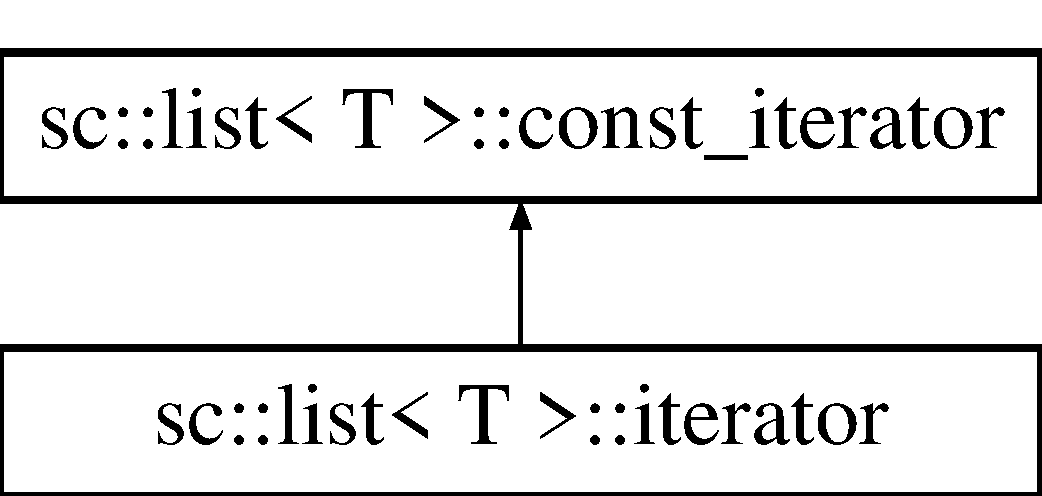
\includegraphics[height=2.000000cm]{classsc_1_1list_1_1const__iterator}
\end{center}
\end{figure}
\subsection*{Public Member Functions}
\begin{DoxyCompactItemize}
\item 
\mbox{\hyperlink{classsc_1_1list_1_1const__iterator_a54f14844dda37c2ebd95c7c6d7fe686d}{const\+\_\+iterator}} ()
\item 
\mbox{\hyperlink{classsc_1_1list_1_1const__iterator_a2a8ca8f4d9e7df000821825d0971c65b}{$\sim$const\+\_\+iterator}} ()=default
\item 
const T \& \mbox{\hyperlink{classsc_1_1list_1_1const__iterator_a24261f681d1a805b5c50a59b3242c0f2}{operator$\ast$}} () const
\item 
\mbox{\hyperlink{classsc_1_1list_1_1const__iterator}{const\+\_\+iterator}} \& \mbox{\hyperlink{classsc_1_1list_1_1const__iterator_abc6d5da99e4c689c662a0037b0bc9013}{operator++}} ()
\item 
\mbox{\hyperlink{classsc_1_1list_1_1const__iterator}{const\+\_\+iterator}} \mbox{\hyperlink{classsc_1_1list_1_1const__iterator_a6b724b61cbc4087c43836dced5eed52f}{operator++}} (int)
\item 
\mbox{\hyperlink{classsc_1_1list_1_1const__iterator}{const\+\_\+iterator}} \& \mbox{\hyperlink{classsc_1_1list_1_1const__iterator_aeb7c02bf76c6734253d09a5e2da94d9f}{operator-\/-\/}} ()
\item 
\mbox{\hyperlink{classsc_1_1list_1_1const__iterator}{const\+\_\+iterator}} \mbox{\hyperlink{classsc_1_1list_1_1const__iterator_aa4b38c471c0754e785c10a2e3aa0bf19}{operator-\/-\/}} (int)
\item 
bool \mbox{\hyperlink{classsc_1_1list_1_1const__iterator_a64650201a32eb1cbc7875e8e7a3434e1}{operator==}} (const \mbox{\hyperlink{classsc_1_1list_1_1const__iterator}{const\+\_\+iterator}} \&rhs) const
\item 
bool \mbox{\hyperlink{classsc_1_1list_1_1const__iterator_a2d271dbabdc3d2e47d1642a5e7beb84d}{operator!=}} (const \mbox{\hyperlink{classsc_1_1list_1_1const__iterator}{const\+\_\+iterator}} \&rhs) const
\end{DoxyCompactItemize}
\subsection*{Protected Member Functions}
\begin{DoxyCompactItemize}
\item 
\mbox{\hyperlink{classsc_1_1list_1_1const__iterator_a72c4f8d017e53d713629bec30ce0d1a9}{const\+\_\+iterator}} (Node $\ast$p)
\item 
T \& \mbox{\hyperlink{classsc_1_1list_1_1const__iterator_acc55cfde0e7405a0b4cf430ccac01a26}{reference}} () const
\end{DoxyCompactItemize}
\subsection*{Protected Attributes}
\begin{DoxyCompactItemize}
\item 
Node $\ast$ \mbox{\hyperlink{classsc_1_1list_1_1const__iterator_ac8a1ecff3dcc804cd3fabfaf2360d461}{current}}
\end{DoxyCompactItemize}
\subsection*{Friends}
\begin{DoxyCompactItemize}
\item 
class \mbox{\hyperlink{classsc_1_1list_1_1const__iterator_ab6cf03d50c50087700b0fb872accfa7b}{list$<$ T $>$}}
\end{DoxyCompactItemize}


\subsection{Detailed Description}
\subsubsection*{template$<$typename T$>$\newline
class sc\+::list$<$ T $>$\+::const\+\_\+iterator}

Classe const iterator, comporta todas as funções que podem ser usadas por iteradores constantes do tipo da lista 

\subsection{Constructor \& Destructor Documentation}
\mbox{\Hypertarget{classsc_1_1list_1_1const__iterator_a54f14844dda37c2ebd95c7c6d7fe686d}\label{classsc_1_1list_1_1const__iterator_a54f14844dda37c2ebd95c7c6d7fe686d}} 
\index{sc\+::list\+::const\+\_\+iterator@{sc\+::list\+::const\+\_\+iterator}!const\+\_\+iterator@{const\+\_\+iterator}}
\index{const\+\_\+iterator@{const\+\_\+iterator}!sc\+::list\+::const\+\_\+iterator@{sc\+::list\+::const\+\_\+iterator}}
\subsubsection{\texorpdfstring{const\+\_\+iterator()}{const\_iterator()}\hspace{0.1cm}{\footnotesize\ttfamily [1/2]}}
{\footnotesize\ttfamily template$<$typename T $>$ \\
list\+::const\+\_\+iterator\+::const\+\_\+iterator (\begin{DoxyParamCaption}{ }\end{DoxyParamCaption})}

Construtor da classe \mbox{\hyperlink{classsc_1_1list_1_1const__iterator}{const\+\_\+iterator}} 
\begin{DoxyParams}{Parameters}
{\em (empty} & and single value) \\
\hline
\end{DoxyParams}
\mbox{\Hypertarget{classsc_1_1list_1_1const__iterator_a2a8ca8f4d9e7df000821825d0971c65b}\label{classsc_1_1list_1_1const__iterator_a2a8ca8f4d9e7df000821825d0971c65b}} 
\index{sc\+::list\+::const\+\_\+iterator@{sc\+::list\+::const\+\_\+iterator}!````~const\+\_\+iterator@{$\sim$const\+\_\+iterator}}
\index{````~const\+\_\+iterator@{$\sim$const\+\_\+iterator}!sc\+::list\+::const\+\_\+iterator@{sc\+::list\+::const\+\_\+iterator}}
\subsubsection{\texorpdfstring{$\sim$const\+\_\+iterator()}{~const\_iterator()}}
{\footnotesize\ttfamily template$<$typename T$>$ \\
\mbox{\hyperlink{classsc_1_1list}{sc\+::list}}$<$ T $>$\+::const\+\_\+iterator\+::$\sim$const\+\_\+iterator (\begin{DoxyParamCaption}{ }\end{DoxyParamCaption})\hspace{0.3cm}{\ttfamily [default]}}

Destrutor da classe \mbox{\hyperlink{classsc_1_1list_1_1const__iterator}{const\+\_\+iterator}} 
\begin{DoxyParams}{Parameters}
{\em (empty} & and single value) \\
\hline
\end{DoxyParams}
\mbox{\Hypertarget{classsc_1_1list_1_1const__iterator_a72c4f8d017e53d713629bec30ce0d1a9}\label{classsc_1_1list_1_1const__iterator_a72c4f8d017e53d713629bec30ce0d1a9}} 
\index{sc\+::list\+::const\+\_\+iterator@{sc\+::list\+::const\+\_\+iterator}!const\+\_\+iterator@{const\+\_\+iterator}}
\index{const\+\_\+iterator@{const\+\_\+iterator}!sc\+::list\+::const\+\_\+iterator@{sc\+::list\+::const\+\_\+iterator}}
\subsubsection{\texorpdfstring{const\+\_\+iterator()}{const\_iterator()}\hspace{0.1cm}{\footnotesize\ttfamily [2/2]}}
{\footnotesize\ttfamily template$<$typename T $>$ \\
list\+::const\+\_\+iterator\+::const\+\_\+iterator (\begin{DoxyParamCaption}\item[{Node $\ast$}]{p }\end{DoxyParamCaption})\hspace{0.3cm}{\ttfamily [protected]}}



\subsection{Member Function Documentation}
\mbox{\Hypertarget{classsc_1_1list_1_1const__iterator_a2d271dbabdc3d2e47d1642a5e7beb84d}\label{classsc_1_1list_1_1const__iterator_a2d271dbabdc3d2e47d1642a5e7beb84d}} 
\index{sc\+::list\+::const\+\_\+iterator@{sc\+::list\+::const\+\_\+iterator}!operator"!=@{operator"!=}}
\index{operator"!=@{operator"!=}!sc\+::list\+::const\+\_\+iterator@{sc\+::list\+::const\+\_\+iterator}}
\subsubsection{\texorpdfstring{operator"!=()}{operator!=()}}
{\footnotesize\ttfamily template$<$typename T $>$ \\
bool list\+::const\+\_\+iterator\+::operator!= (\begin{DoxyParamCaption}\item[{const \mbox{\hyperlink{classsc_1_1list_1_1const__iterator}{const\+\_\+iterator}} \&}]{rhs }\end{DoxyParamCaption}) const}

\mbox{\Hypertarget{classsc_1_1list_1_1const__iterator_a24261f681d1a805b5c50a59b3242c0f2}\label{classsc_1_1list_1_1const__iterator_a24261f681d1a805b5c50a59b3242c0f2}} 
\index{sc\+::list\+::const\+\_\+iterator@{sc\+::list\+::const\+\_\+iterator}!operator$\ast$@{operator$\ast$}}
\index{operator$\ast$@{operator$\ast$}!sc\+::list\+::const\+\_\+iterator@{sc\+::list\+::const\+\_\+iterator}}
\subsubsection{\texorpdfstring{operator$\ast$()}{operator*()}}
{\footnotesize\ttfamily template$<$typename T $>$ \\
const T \& list\+::const\+\_\+iterator\+::operator$\ast$ (\begin{DoxyParamCaption}{ }\end{DoxyParamCaption}) const}

Operador $\ast$ da classe \mbox{\hyperlink{classsc_1_1list_1_1const__iterator}{const\+\_\+iterator}} 
\begin{DoxyParams}{Parameters}
{\em (void)} & \\
\hline
\end{DoxyParams}
\begin{DoxyReturn}{Returns}
value 
\end{DoxyReturn}
\mbox{\Hypertarget{classsc_1_1list_1_1const__iterator_abc6d5da99e4c689c662a0037b0bc9013}\label{classsc_1_1list_1_1const__iterator_abc6d5da99e4c689c662a0037b0bc9013}} 
\index{sc\+::list\+::const\+\_\+iterator@{sc\+::list\+::const\+\_\+iterator}!operator++@{operator++}}
\index{operator++@{operator++}!sc\+::list\+::const\+\_\+iterator@{sc\+::list\+::const\+\_\+iterator}}
\subsubsection{\texorpdfstring{operator++()}{operator++()}\hspace{0.1cm}{\footnotesize\ttfamily [1/2]}}
{\footnotesize\ttfamily template$<$typename T $>$ \\
\mbox{\hyperlink{classsc_1_1list}{list}}$<$ T $>$\+::\mbox{\hyperlink{classsc_1_1list_1_1const__iterator}{const\+\_\+iterator}} \& list\+::const\+\_\+iterator\+::operator++ (\begin{DoxyParamCaption}{ }\end{DoxyParamCaption})}

Operador ++it da classe \mbox{\hyperlink{classsc_1_1list_1_1const__iterator}{const\+\_\+iterator}} 
\begin{DoxyParams}{Parameters}
{\em (void)} & \\
\hline
\end{DoxyParams}
\begin{DoxyReturn}{Returns}
reference 
\end{DoxyReturn}
\mbox{\Hypertarget{classsc_1_1list_1_1const__iterator_a6b724b61cbc4087c43836dced5eed52f}\label{classsc_1_1list_1_1const__iterator_a6b724b61cbc4087c43836dced5eed52f}} 
\index{sc\+::list\+::const\+\_\+iterator@{sc\+::list\+::const\+\_\+iterator}!operator++@{operator++}}
\index{operator++@{operator++}!sc\+::list\+::const\+\_\+iterator@{sc\+::list\+::const\+\_\+iterator}}
\subsubsection{\texorpdfstring{operator++()}{operator++()}\hspace{0.1cm}{\footnotesize\ttfamily [2/2]}}
{\footnotesize\ttfamily template$<$typename T $>$ \\
\mbox{\hyperlink{classsc_1_1list}{list}}$<$ T $>$\+::\mbox{\hyperlink{classsc_1_1list_1_1const__iterator}{const\+\_\+iterator}} list\+::const\+\_\+iterator\+::operator++ (\begin{DoxyParamCaption}\item[{int}]{ }\end{DoxyParamCaption})}

Operador it++ da classe \mbox{\hyperlink{classsc_1_1list_1_1const__iterator}{const\+\_\+iterator}} 
\begin{DoxyParams}{Parameters}
{\em (void)} & \\
\hline
\end{DoxyParams}
\begin{DoxyReturn}{Returns}
reference 
\end{DoxyReturn}
\mbox{\Hypertarget{classsc_1_1list_1_1const__iterator_aeb7c02bf76c6734253d09a5e2da94d9f}\label{classsc_1_1list_1_1const__iterator_aeb7c02bf76c6734253d09a5e2da94d9f}} 
\index{sc\+::list\+::const\+\_\+iterator@{sc\+::list\+::const\+\_\+iterator}!operator-\/-\/@{operator-\/-\/}}
\index{operator-\/-\/@{operator-\/-\/}!sc\+::list\+::const\+\_\+iterator@{sc\+::list\+::const\+\_\+iterator}}
\subsubsection{\texorpdfstring{operator-\/-\/()}{operator--()}\hspace{0.1cm}{\footnotesize\ttfamily [1/2]}}
{\footnotesize\ttfamily template$<$typename T $>$ \\
\mbox{\hyperlink{classsc_1_1list}{list}}$<$ T $>$\+::\mbox{\hyperlink{classsc_1_1list_1_1const__iterator}{const\+\_\+iterator}} \& list\+::const\+\_\+iterator\+::operator-\/-\/ (\begin{DoxyParamCaption}{ }\end{DoxyParamCaption})}

Operador --it da classe \mbox{\hyperlink{classsc_1_1list_1_1const__iterator}{const\+\_\+iterator}} 
\begin{DoxyParams}{Parameters}
{\em (void)} & \\
\hline
\end{DoxyParams}
\begin{DoxyReturn}{Returns}
reference 
\end{DoxyReturn}
\mbox{\Hypertarget{classsc_1_1list_1_1const__iterator_aa4b38c471c0754e785c10a2e3aa0bf19}\label{classsc_1_1list_1_1const__iterator_aa4b38c471c0754e785c10a2e3aa0bf19}} 
\index{sc\+::list\+::const\+\_\+iterator@{sc\+::list\+::const\+\_\+iterator}!operator-\/-\/@{operator-\/-\/}}
\index{operator-\/-\/@{operator-\/-\/}!sc\+::list\+::const\+\_\+iterator@{sc\+::list\+::const\+\_\+iterator}}
\subsubsection{\texorpdfstring{operator-\/-\/()}{operator--()}\hspace{0.1cm}{\footnotesize\ttfamily [2/2]}}
{\footnotesize\ttfamily template$<$typename T $>$ \\
\mbox{\hyperlink{classsc_1_1list}{list}}$<$ T $>$\+::\mbox{\hyperlink{classsc_1_1list_1_1const__iterator}{const\+\_\+iterator}} list\+::const\+\_\+iterator\+::operator-\/-\/ (\begin{DoxyParamCaption}\item[{int}]{ }\end{DoxyParamCaption})}

Operador it-- da classe \mbox{\hyperlink{classsc_1_1list_1_1const__iterator}{const\+\_\+iterator}} 
\begin{DoxyParams}{Parameters}
{\em (void)} & \\
\hline
\end{DoxyParams}
\begin{DoxyReturn}{Returns}
reference 
\end{DoxyReturn}
\mbox{\Hypertarget{classsc_1_1list_1_1const__iterator_a64650201a32eb1cbc7875e8e7a3434e1}\label{classsc_1_1list_1_1const__iterator_a64650201a32eb1cbc7875e8e7a3434e1}} 
\index{sc\+::list\+::const\+\_\+iterator@{sc\+::list\+::const\+\_\+iterator}!operator==@{operator==}}
\index{operator==@{operator==}!sc\+::list\+::const\+\_\+iterator@{sc\+::list\+::const\+\_\+iterator}}
\subsubsection{\texorpdfstring{operator==()}{operator==()}}
{\footnotesize\ttfamily template$<$typename T $>$ \\
bool list\+::const\+\_\+iterator\+::operator== (\begin{DoxyParamCaption}\item[{const \mbox{\hyperlink{classsc_1_1list_1_1const__iterator}{const\+\_\+iterator}} \&}]{rhs }\end{DoxyParamCaption}) const}

$<$ Operador == da classe \mbox{\hyperlink{classsc_1_1list_1_1const__iterator}{const\+\_\+iterator}} 
\begin{DoxyParams}{Parameters}
{\em (const} & iterator\& rhs) \\
\hline
\end{DoxyParams}
\begin{DoxyReturn}{Returns}
boolean  Operador != da classe \mbox{\hyperlink{classsc_1_1list_1_1const__iterator}{const\+\_\+iterator}} 
\end{DoxyReturn}

\begin{DoxyParams}{Parameters}
{\em (const} & iterator\& rhs) \\
\hline
\end{DoxyParams}
\begin{DoxyReturn}{Returns}
boolean 
\end{DoxyReturn}
\mbox{\Hypertarget{classsc_1_1list_1_1const__iterator_acc55cfde0e7405a0b4cf430ccac01a26}\label{classsc_1_1list_1_1const__iterator_acc55cfde0e7405a0b4cf430ccac01a26}} 
\index{sc\+::list\+::const\+\_\+iterator@{sc\+::list\+::const\+\_\+iterator}!reference@{reference}}
\index{reference@{reference}!sc\+::list\+::const\+\_\+iterator@{sc\+::list\+::const\+\_\+iterator}}
\subsubsection{\texorpdfstring{reference()}{reference()}}
{\footnotesize\ttfamily template$<$typename T $>$ \\
T \& list\+::const\+\_\+iterator\+::reference (\begin{DoxyParamCaption}{ }\end{DoxyParamCaption}) const\hspace{0.3cm}{\ttfamily [protected]}}



\subsection{Friends And Related Function Documentation}
\mbox{\Hypertarget{classsc_1_1list_1_1const__iterator_ab6cf03d50c50087700b0fb872accfa7b}\label{classsc_1_1list_1_1const__iterator_ab6cf03d50c50087700b0fb872accfa7b}} 
\index{sc\+::list\+::const\+\_\+iterator@{sc\+::list\+::const\+\_\+iterator}!list$<$ T $>$@{list$<$ T $>$}}
\index{list$<$ T $>$@{list$<$ T $>$}!sc\+::list\+::const\+\_\+iterator@{sc\+::list\+::const\+\_\+iterator}}
\subsubsection{\texorpdfstring{list$<$ T $>$}{list< T >}}
{\footnotesize\ttfamily template$<$typename T$>$ \\
friend class \mbox{\hyperlink{classsc_1_1list}{list}}$<$ T $>$\hspace{0.3cm}{\ttfamily [friend]}}



\subsection{Member Data Documentation}
\mbox{\Hypertarget{classsc_1_1list_1_1const__iterator_ac8a1ecff3dcc804cd3fabfaf2360d461}\label{classsc_1_1list_1_1const__iterator_ac8a1ecff3dcc804cd3fabfaf2360d461}} 
\index{sc\+::list\+::const\+\_\+iterator@{sc\+::list\+::const\+\_\+iterator}!current@{current}}
\index{current@{current}!sc\+::list\+::const\+\_\+iterator@{sc\+::list\+::const\+\_\+iterator}}
\subsubsection{\texorpdfstring{current}{current}}
{\footnotesize\ttfamily template$<$typename T$>$ \\
Node$\ast$ \mbox{\hyperlink{classsc_1_1list}{sc\+::list}}$<$ T $>$\+::const\+\_\+iterator\+::current\hspace{0.3cm}{\ttfamily [protected]}}



The documentation for this class was generated from the following files\+:\begin{DoxyCompactItemize}
\item 
include/\mbox{\hyperlink{list_8hpp}{list.\+hpp}}\item 
include/\mbox{\hyperlink{list_8inl}{list.\+inl}}\end{DoxyCompactItemize}

\hypertarget{classsc_1_1list_1_1iterator}{}\section{sc\+:\+:list$<$ T $>$\+:\+:iterator Class Reference}
\label{classsc_1_1list_1_1iterator}\index{sc\+::list$<$ T $>$\+::iterator@{sc\+::list$<$ T $>$\+::iterator}}


{\ttfamily \#include $<$list.\+hpp$>$}

Inheritance diagram for sc\+:\+:list$<$ T $>$\+:\+:iterator\+:\begin{figure}[H]
\begin{center}
\leavevmode
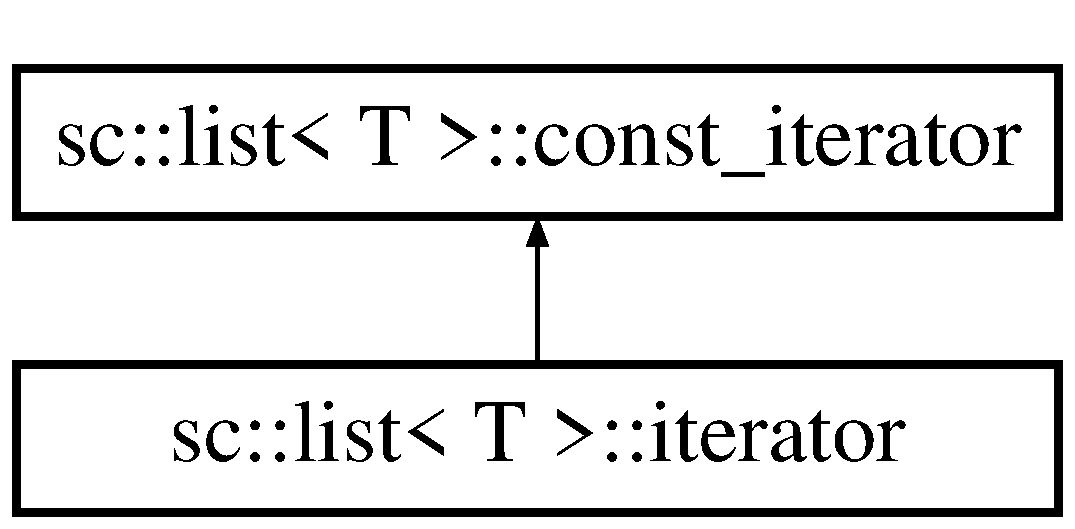
\includegraphics[height=2.000000cm]{classsc_1_1list_1_1iterator}
\end{center}
\end{figure}
\subsection*{Public Member Functions}
\begin{DoxyCompactItemize}
\item 
\mbox{\hyperlink{classsc_1_1list_1_1iterator_acd90feec03d8a2762f36407a27166bb9}{iterator}} ()
\item 
\mbox{\hyperlink{classsc_1_1list_1_1iterator_a84674835b45ab08a280df0c6a474b57a}{$\sim$iterator}} ()=default
\item 
const T \& \mbox{\hyperlink{classsc_1_1list_1_1iterator_a8e1feb979567a3fa27add54563d0008f}{operator$\ast$}} () const
\item 
T \& \mbox{\hyperlink{classsc_1_1list_1_1iterator_a302efc11d84340a0f69090c001c19b79}{operator$\ast$}} ()
\item 
\mbox{\hyperlink{classsc_1_1list_1_1iterator}{iterator}} \& \mbox{\hyperlink{classsc_1_1list_1_1iterator_a1853e5deff88ddd275f51b366971de17}{operator++}} ()
\item 
\mbox{\hyperlink{classsc_1_1list_1_1iterator}{iterator}} \mbox{\hyperlink{classsc_1_1list_1_1iterator_a07136b928446a99cfb298e631ab0e07e}{operator++}} (int)
\item 
\mbox{\hyperlink{classsc_1_1list_1_1iterator}{iterator}} \& \mbox{\hyperlink{classsc_1_1list_1_1iterator_a2780ff54bf392eb23811ca9b7d116908}{operator-\/-\/}} ()
\item 
\mbox{\hyperlink{classsc_1_1list_1_1iterator}{iterator}} \mbox{\hyperlink{classsc_1_1list_1_1iterator_ae0508132c274454f7199eb801a28f4e9}{operator-\/-\/}} (int)
\end{DoxyCompactItemize}
\subsection*{Protected Member Functions}
\begin{DoxyCompactItemize}
\item 
\mbox{\hyperlink{classsc_1_1list_1_1iterator_a818795d7651516a93e563f3229e86351}{iterator}} (Node $\ast$p)
\end{DoxyCompactItemize}
\subsection*{Friends}
\begin{DoxyCompactItemize}
\item 
class \mbox{\hyperlink{classsc_1_1list_1_1iterator_ab6cf03d50c50087700b0fb872accfa7b}{list$<$ T $>$}}
\end{DoxyCompactItemize}
\subsection*{Additional Inherited Members}


\subsection{Detailed Description}
\subsubsection*{template$<$typename T$>$\newline
class sc\+::list$<$ T $>$\+::iterator}

Classe iterator, comporta todas as funções que podem ser usadas por iteradores do tipo da lista 

\subsection{Constructor \& Destructor Documentation}
\mbox{\Hypertarget{classsc_1_1list_1_1iterator_acd90feec03d8a2762f36407a27166bb9}\label{classsc_1_1list_1_1iterator_acd90feec03d8a2762f36407a27166bb9}} 
\index{sc\+::list\+::iterator@{sc\+::list\+::iterator}!iterator@{iterator}}
\index{iterator@{iterator}!sc\+::list\+::iterator@{sc\+::list\+::iterator}}
\subsubsection{\texorpdfstring{iterator()}{iterator()}\hspace{0.1cm}{\footnotesize\ttfamily [1/2]}}
{\footnotesize\ttfamily template$<$typename T$>$ \\
\mbox{\hyperlink{classsc_1_1list}{sc\+::list}}$<$ T $>$\+::iterator\+::iterator (\begin{DoxyParamCaption}{ }\end{DoxyParamCaption})\hspace{0.3cm}{\ttfamily [inline]}}

Construtor da classe iterator 
\begin{DoxyParams}{Parameters}
{\em (empty} & and single value) \\
\hline
\end{DoxyParams}
\mbox{\Hypertarget{classsc_1_1list_1_1iterator_a84674835b45ab08a280df0c6a474b57a}\label{classsc_1_1list_1_1iterator_a84674835b45ab08a280df0c6a474b57a}} 
\index{sc\+::list\+::iterator@{sc\+::list\+::iterator}!````~iterator@{$\sim$iterator}}
\index{````~iterator@{$\sim$iterator}!sc\+::list\+::iterator@{sc\+::list\+::iterator}}
\subsubsection{\texorpdfstring{$\sim$iterator()}{~iterator()}}
{\footnotesize\ttfamily template$<$typename T$>$ \\
\mbox{\hyperlink{classsc_1_1list}{sc\+::list}}$<$ T $>$\+::iterator\+::$\sim$iterator (\begin{DoxyParamCaption}{ }\end{DoxyParamCaption})\hspace{0.3cm}{\ttfamily [default]}}

Destrutor da classe iterator 
\begin{DoxyParams}{Parameters}
{\em (empty} & and single value) \\
\hline
\end{DoxyParams}
\mbox{\Hypertarget{classsc_1_1list_1_1iterator_a818795d7651516a93e563f3229e86351}\label{classsc_1_1list_1_1iterator_a818795d7651516a93e563f3229e86351}} 
\index{sc\+::list\+::iterator@{sc\+::list\+::iterator}!iterator@{iterator}}
\index{iterator@{iterator}!sc\+::list\+::iterator@{sc\+::list\+::iterator}}
\subsubsection{\texorpdfstring{iterator()}{iterator()}\hspace{0.1cm}{\footnotesize\ttfamily [2/2]}}
{\footnotesize\ttfamily template$<$typename T$>$ \\
\mbox{\hyperlink{classsc_1_1list}{sc\+::list}}$<$ T $>$\+::iterator\+::iterator (\begin{DoxyParamCaption}\item[{Node $\ast$}]{p }\end{DoxyParamCaption})\hspace{0.3cm}{\ttfamily [inline]}, {\ttfamily [protected]}}



\subsection{Member Function Documentation}
\mbox{\Hypertarget{classsc_1_1list_1_1iterator_a8e1feb979567a3fa27add54563d0008f}\label{classsc_1_1list_1_1iterator_a8e1feb979567a3fa27add54563d0008f}} 
\index{sc\+::list\+::iterator@{sc\+::list\+::iterator}!operator$\ast$@{operator$\ast$}}
\index{operator$\ast$@{operator$\ast$}!sc\+::list\+::iterator@{sc\+::list\+::iterator}}
\subsubsection{\texorpdfstring{operator$\ast$()}{operator*()}\hspace{0.1cm}{\footnotesize\ttfamily [1/2]}}
{\footnotesize\ttfamily template$<$typename T$>$ \\
const T\& \mbox{\hyperlink{classsc_1_1list}{sc\+::list}}$<$ T $>$\+::iterator\+::operator$\ast$ (\begin{DoxyParamCaption}{ }\end{DoxyParamCaption}) const}

Operador $\ast$ da classe iterator 
\begin{DoxyParams}{Parameters}
{\em (void)} & \\
\hline
\end{DoxyParams}
\begin{DoxyReturn}{Returns}
value 
\end{DoxyReturn}
\mbox{\Hypertarget{classsc_1_1list_1_1iterator_a302efc11d84340a0f69090c001c19b79}\label{classsc_1_1list_1_1iterator_a302efc11d84340a0f69090c001c19b79}} 
\index{sc\+::list\+::iterator@{sc\+::list\+::iterator}!operator$\ast$@{operator$\ast$}}
\index{operator$\ast$@{operator$\ast$}!sc\+::list\+::iterator@{sc\+::list\+::iterator}}
\subsubsection{\texorpdfstring{operator$\ast$()}{operator*()}\hspace{0.1cm}{\footnotesize\ttfamily [2/2]}}
{\footnotesize\ttfamily template$<$typename T $>$ \\
T \& list\+::iterator\+::operator$\ast$ (\begin{DoxyParamCaption}{ }\end{DoxyParamCaption})}

\mbox{\Hypertarget{classsc_1_1list_1_1iterator_a1853e5deff88ddd275f51b366971de17}\label{classsc_1_1list_1_1iterator_a1853e5deff88ddd275f51b366971de17}} 
\index{sc\+::list\+::iterator@{sc\+::list\+::iterator}!operator++@{operator++}}
\index{operator++@{operator++}!sc\+::list\+::iterator@{sc\+::list\+::iterator}}
\subsubsection{\texorpdfstring{operator++()}{operator++()}\hspace{0.1cm}{\footnotesize\ttfamily [1/2]}}
{\footnotesize\ttfamily template$<$typename T $>$ \\
\mbox{\hyperlink{classsc_1_1list}{list}}$<$ T $>$\+::\mbox{\hyperlink{classsc_1_1list_1_1iterator}{iterator}} \& list\+::iterator\+::operator++ (\begin{DoxyParamCaption}{ }\end{DoxyParamCaption})}

Operador ++it da classe iterator 
\begin{DoxyParams}{Parameters}
{\em (void)} & \\
\hline
\end{DoxyParams}
\begin{DoxyReturn}{Returns}
reference 
\end{DoxyReturn}
\mbox{\Hypertarget{classsc_1_1list_1_1iterator_a07136b928446a99cfb298e631ab0e07e}\label{classsc_1_1list_1_1iterator_a07136b928446a99cfb298e631ab0e07e}} 
\index{sc\+::list\+::iterator@{sc\+::list\+::iterator}!operator++@{operator++}}
\index{operator++@{operator++}!sc\+::list\+::iterator@{sc\+::list\+::iterator}}
\subsubsection{\texorpdfstring{operator++()}{operator++()}\hspace{0.1cm}{\footnotesize\ttfamily [2/2]}}
{\footnotesize\ttfamily template$<$typename T $>$ \\
\mbox{\hyperlink{classsc_1_1list}{list}}$<$ T $>$\+::\mbox{\hyperlink{classsc_1_1list_1_1iterator}{iterator}} list\+::iterator\+::operator++ (\begin{DoxyParamCaption}\item[{int}]{ }\end{DoxyParamCaption})}

Operador it++ da classe iterator 
\begin{DoxyParams}{Parameters}
{\em (void)} & \\
\hline
\end{DoxyParams}
\begin{DoxyReturn}{Returns}
reference 
\end{DoxyReturn}
\mbox{\Hypertarget{classsc_1_1list_1_1iterator_a2780ff54bf392eb23811ca9b7d116908}\label{classsc_1_1list_1_1iterator_a2780ff54bf392eb23811ca9b7d116908}} 
\index{sc\+::list\+::iterator@{sc\+::list\+::iterator}!operator-\/-\/@{operator-\/-\/}}
\index{operator-\/-\/@{operator-\/-\/}!sc\+::list\+::iterator@{sc\+::list\+::iterator}}
\subsubsection{\texorpdfstring{operator-\/-\/()}{operator--()}\hspace{0.1cm}{\footnotesize\ttfamily [1/2]}}
{\footnotesize\ttfamily template$<$typename T $>$ \\
\mbox{\hyperlink{classsc_1_1list}{list}}$<$ T $>$\+::\mbox{\hyperlink{classsc_1_1list_1_1iterator}{iterator}} \& list\+::iterator\+::operator-\/-\/ (\begin{DoxyParamCaption}{ }\end{DoxyParamCaption})}

Operador --it da classe iterator 
\begin{DoxyParams}{Parameters}
{\em (void)} & \\
\hline
\end{DoxyParams}
\begin{DoxyReturn}{Returns}
reference 
\end{DoxyReturn}
\mbox{\Hypertarget{classsc_1_1list_1_1iterator_ae0508132c274454f7199eb801a28f4e9}\label{classsc_1_1list_1_1iterator_ae0508132c274454f7199eb801a28f4e9}} 
\index{sc\+::list\+::iterator@{sc\+::list\+::iterator}!operator-\/-\/@{operator-\/-\/}}
\index{operator-\/-\/@{operator-\/-\/}!sc\+::list\+::iterator@{sc\+::list\+::iterator}}
\subsubsection{\texorpdfstring{operator-\/-\/()}{operator--()}\hspace{0.1cm}{\footnotesize\ttfamily [2/2]}}
{\footnotesize\ttfamily template$<$typename T $>$ \\
\mbox{\hyperlink{classsc_1_1list}{list}}$<$ T $>$\+::\mbox{\hyperlink{classsc_1_1list_1_1iterator}{iterator}} list\+::iterator\+::operator-\/-\/ (\begin{DoxyParamCaption}\item[{int}]{ }\end{DoxyParamCaption})}

Operador it-- da classe iterator 
\begin{DoxyParams}{Parameters}
{\em (void)} & \\
\hline
\end{DoxyParams}
\begin{DoxyReturn}{Returns}
reference 
\end{DoxyReturn}


\subsection{Friends And Related Function Documentation}
\mbox{\Hypertarget{classsc_1_1list_1_1iterator_ab6cf03d50c50087700b0fb872accfa7b}\label{classsc_1_1list_1_1iterator_ab6cf03d50c50087700b0fb872accfa7b}} 
\index{sc\+::list\+::iterator@{sc\+::list\+::iterator}!list$<$ T $>$@{list$<$ T $>$}}
\index{list$<$ T $>$@{list$<$ T $>$}!sc\+::list\+::iterator@{sc\+::list\+::iterator}}
\subsubsection{\texorpdfstring{list$<$ T $>$}{list< T >}}
{\footnotesize\ttfamily template$<$typename T$>$ \\
friend class \mbox{\hyperlink{classsc_1_1list}{list}}$<$ T $>$\hspace{0.3cm}{\ttfamily [friend]}}



The documentation for this class was generated from the following files\+:\begin{DoxyCompactItemize}
\item 
include/\mbox{\hyperlink{list_8hpp}{list.\+hpp}}\item 
include/\mbox{\hyperlink{list_8inl}{list.\+inl}}\end{DoxyCompactItemize}

\hypertarget{classsc_1_1list}{}\section{sc\+:\+:list$<$ T $>$ Class Template Reference}
\label{classsc_1_1list}\index{sc\+::list$<$ T $>$@{sc\+::list$<$ T $>$}}


{\ttfamily \#include $<$list.\+hpp$>$}

\subsection*{Classes}
\begin{DoxyCompactItemize}
\item 
class \mbox{\hyperlink{classsc_1_1list_1_1const__iterator}{const\+\_\+iterator}}
\item 
class \mbox{\hyperlink{classsc_1_1list_1_1iterator}{iterator}}
\end{DoxyCompactItemize}
\subsection*{Public Member Functions}
\begin{DoxyCompactItemize}
\item 
\mbox{\hyperlink{classsc_1_1list_ac7b95807230114dc58f2b1156cb3cdba}{list}} ()
\item 
\mbox{\hyperlink{classsc_1_1list_a154e0a43ee70faa49f66f9ce4ce48583}{list}} (size\+\_\+t count)
\item 
{\footnotesize template$<$typename Input\+It $>$ }\\\mbox{\hyperlink{classsc_1_1list_a142545a98bc5fec38606bf7000620864}{list}} (Input\+It first, Input\+It last)
\item 
\mbox{\hyperlink{classsc_1_1list_a1fe5b60798e979cb0a5b1663d64ec69b}{list}} (const \mbox{\hyperlink{classsc_1_1list}{list}} \&other)
\item 
\mbox{\hyperlink{classsc_1_1list_ae85152bcf538c929944790b1c30d3b22}{list}} (std\+::initializer\+\_\+list$<$ T $>$ ilist)
\item 
\mbox{\hyperlink{classsc_1_1list_a72eaabb03a048506432f8d167db12524}{$\sim$list}} ()
\item 
\mbox{\hyperlink{classsc_1_1list}{list}} \& \mbox{\hyperlink{classsc_1_1list_a09a75038c91f224b930fc63b39c4ad56}{operator=}} (const \mbox{\hyperlink{classsc_1_1list}{list}} \&other)
\item 
\mbox{\hyperlink{classsc_1_1list}{list}} \& \mbox{\hyperlink{classsc_1_1list_a480d22198a20823cf386bc3caef22cae}{operator=}} (std\+::initializer\+\_\+list$<$ T $>$ ilist)
\item 
\mbox{\hyperlink{classsc_1_1list_1_1iterator}{iterator}} \mbox{\hyperlink{classsc_1_1list_a5f5e6470de04a47d530dae0c87403caa}{begin}} ()
\item 
\mbox{\hyperlink{classsc_1_1list_1_1const__iterator}{const\+\_\+iterator}} \mbox{\hyperlink{classsc_1_1list_aff238d93b985d8e0c340519c58e378cf}{cbegin}} () const
\item 
\mbox{\hyperlink{classsc_1_1list_1_1iterator}{iterator}} \mbox{\hyperlink{classsc_1_1list_a31c42556b18886277d436ec540019349}{end}} ()
\item 
\mbox{\hyperlink{classsc_1_1list_1_1const__iterator}{const\+\_\+iterator}} \mbox{\hyperlink{classsc_1_1list_a935b1947e028c0f733bbe14afd0fd38f}{cend}} () const
\item 
int \mbox{\hyperlink{classsc_1_1list_ae7dcc01498f6def3ffff29a35b36c2f3}{size}} () const
\item 
bool \mbox{\hyperlink{classsc_1_1list_aeb4d6c3d1fc142b0ff35a3ec203b7b3f}{empty}} () const
\item 
void \mbox{\hyperlink{classsc_1_1list_a86207fd2b1a6355882e0f1c581b5bc65}{push\+\_\+back}} (const T \&value)
\item 
void \mbox{\hyperlink{classsc_1_1list_aff098c381e8ad50e58c20c668d4d5d77}{push\+\_\+front}} (const T \&value)
\item 
void \mbox{\hyperlink{classsc_1_1list_a0e208afb64eed97d8d9d9315ba211f3c}{pop\+\_\+back}} ()
\item 
void \mbox{\hyperlink{classsc_1_1list_a4e0d8595c1bd85d33a503fbc7bfe6940}{pop\+\_\+front}} ()
\item 
const T \& \mbox{\hyperlink{classsc_1_1list_a57f6bddf67f5d60b5d3293150fbb52a6}{back}} () const
\item 
const T \& \mbox{\hyperlink{classsc_1_1list_a15e1380ab91bf786fa4b34b802d66c0b}{front}} () const
\item 
void \mbox{\hyperlink{classsc_1_1list_ada3f13df5cabc23e702baa64f1b5f76e}{clear}} ()
\item 
bool \mbox{\hyperlink{classsc_1_1list_a36a0bdec0e219977b7f36bf1665fea35}{operator==}} (const \mbox{\hyperlink{classsc_1_1list}{list}}$<$ T $>$ \&rhs)
\item 
bool \mbox{\hyperlink{classsc_1_1list_add9f9d9fb6302969e9ac7822e46ff222}{operator!=}} (const \mbox{\hyperlink{classsc_1_1list}{list}}$<$ T $>$ \&rhs)
\item 
\mbox{\hyperlink{classsc_1_1list_1_1iterator}{iterator}} \mbox{\hyperlink{classsc_1_1list_a12a195a7ebaf3455f245caa852b44a9b}{erase}} (\mbox{\hyperlink{classsc_1_1list_1_1iterator}{iterator}} pos)
\item 
\mbox{\hyperlink{classsc_1_1list_1_1iterator}{iterator}} \mbox{\hyperlink{classsc_1_1list_ae796301c82f58d72d10ec7c30fb0b024}{erase}} (\mbox{\hyperlink{classsc_1_1list_1_1iterator}{iterator}} first, \mbox{\hyperlink{classsc_1_1list_1_1iterator}{iterator}} last)
\item 
{\footnotesize template$<$typename Input\+It $>$ }\\void \mbox{\hyperlink{classsc_1_1list_a5886cd0296e187a96777dd837eaed99b}{assign}} (Input\+It first, Input\+It last)
\item 
void \mbox{\hyperlink{classsc_1_1list_a495ac9f4a80b40ba7d37e6badf24445f}{assign}} (std\+::initializer\+\_\+list$<$ T $>$ ilist)
\item 
void \mbox{\hyperlink{classsc_1_1list_a3578c78367327dba848baa746882640a}{assign}} (size\+\_\+type count, const T \&value)
\item 
\mbox{\hyperlink{classsc_1_1list_1_1iterator}{iterator}} \mbox{\hyperlink{classsc_1_1list_a633565e547a05308a6f527a0aac716f8}{insert}} (\mbox{\hyperlink{classsc_1_1list_1_1iterator}{iterator}} pos, const T \&value)
\item 
\mbox{\hyperlink{classsc_1_1list_1_1iterator}{iterator}} \mbox{\hyperlink{classsc_1_1list_a80098f156b61ebe5555a2d7762507817}{insert}} (\mbox{\hyperlink{classsc_1_1list_1_1iterator}{iterator}} pos, std\+::initializer\+\_\+list$<$ T $>$ ilist)
\item 
{\footnotesize template$<$typename In\+Itr $>$ }\\\mbox{\hyperlink{classsc_1_1list_1_1iterator}{iterator}} \mbox{\hyperlink{classsc_1_1list_a50f5e86e5e8e4bce9ea2401a38a4719a}{insert}} (\mbox{\hyperlink{classsc_1_1list_1_1iterator}{iterator}} pos, In\+Itr first, In\+Itr last)
\item 
{\footnotesize template$<$typename Input\+It $>$ }\\\mbox{\hyperlink{classsc_1_1list}{list}}$<$ T $>$\+::\mbox{\hyperlink{classsc_1_1list_1_1iterator}{iterator}} \mbox{\hyperlink{classsc_1_1list_ad26f50a102e4f66e4d0771bd602fa5f8}{insert}} (\mbox{\hyperlink{classsc_1_1list_1_1iterator}{iterator}} pos, Input\+It first, Input\+It last)
\item 
{\footnotesize template$<$typename T $>$ }\\\mbox{\hyperlink{classsc_1_1list_a242ae734432dc0e8a59dc727ed61d1e6}{list}} (void)
\item 
{\footnotesize template$<$typename T $>$ }\\\mbox{\hyperlink{classsc_1_1list_a679021f4ab00ef04f89ed5567a917f70}{list}} (size\+\_\+t count)
\item 
{\footnotesize template$<$typename Input\+It $>$ }\\\mbox{\hyperlink{classsc_1_1list_a142545a98bc5fec38606bf7000620864}{list}} (Input\+It first, Input\+It last)
\item 
{\footnotesize template$<$typename T $>$ }\\\mbox{\hyperlink{classsc_1_1list_ac2a2da400f459b541ff839cae88a5d99}{list}} (const \mbox{\hyperlink{classsc_1_1list}{list}} \&other)
\item 
{\footnotesize template$<$typename T $>$ }\\\mbox{\hyperlink{classsc_1_1list_a1ebf25d397d69908199b7e25edacf16b}{list}} (std\+::initializer\+\_\+list$<$ T $>$ ilist)
\item 
{\footnotesize template$<$typename Input\+It $>$ }\\void \mbox{\hyperlink{classsc_1_1list_a5886cd0296e187a96777dd837eaed99b}{assign}} (Input\+It first, Input\+It last)
\item 
{\footnotesize template$<$typename T $>$ }\\void \mbox{\hyperlink{classsc_1_1list_a4aa5ed764ec08bf8250d5dc65df8d4a5}{assign}} (std\+::initializer\+\_\+list$<$ T $>$ ilist)
\item 
{\footnotesize template$<$typename T $>$ }\\void \mbox{\hyperlink{classsc_1_1list_ac1e81764b779171186a3970cb1b3d288}{assign}} (size\+\_\+type count, const T \&value)
\item 
{\footnotesize template$<$typename T $>$ }\\\mbox{\hyperlink{classsc_1_1list}{list}}$<$ T $>$\+::\mbox{\hyperlink{classsc_1_1list_1_1iterator}{iterator}} \mbox{\hyperlink{classsc_1_1list_a31f318aea55ddfb39b23370c3a609400}{insert}} (\mbox{\hyperlink{classsc_1_1list_1_1iterator}{iterator}} itr, const T \&value)
\item 
{\footnotesize template$<$typename Input\+It $>$ }\\\mbox{\hyperlink{classsc_1_1list}{list}}$<$ T $>$\+::\mbox{\hyperlink{classsc_1_1list_1_1iterator}{iterator}} \mbox{\hyperlink{classsc_1_1list_ad26f50a102e4f66e4d0771bd602fa5f8}{insert}} (\mbox{\hyperlink{classsc_1_1list_1_1iterator}{iterator}} pos, Input\+It first, Input\+It last)
\item 
{\footnotesize template$<$typename T $>$ }\\\mbox{\hyperlink{classsc_1_1list}{list}}$<$ T $>$\+::\mbox{\hyperlink{classsc_1_1list_1_1iterator}{iterator}} \mbox{\hyperlink{classsc_1_1list_a08e432de3c38c6e770e9c6de2f0782e2}{insert}} (\mbox{\hyperlink{classsc_1_1list_1_1iterator}{iterator}} pos, std\+::initializer\+\_\+list$<$ T $>$ ilist)
\end{DoxyCompactItemize}


\subsection{Detailed Description}
\subsubsection*{template$<$typename T$>$\newline
class sc\+::list$<$ T $>$}

Classe list, comporta todas as funções que podem ser usadas e demais classes de iteradores de tipo abstrato 

\subsection{Constructor \& Destructor Documentation}
\mbox{\Hypertarget{classsc_1_1list_ac7b95807230114dc58f2b1156cb3cdba}\label{classsc_1_1list_ac7b95807230114dc58f2b1156cb3cdba}} 
\index{sc\+::list@{sc\+::list}!list@{list}}
\index{list@{list}!sc\+::list@{sc\+::list}}
\subsubsection{\texorpdfstring{list()}{list()}\hspace{0.1cm}{\footnotesize\ttfamily [1/10]}}
{\footnotesize\ttfamily template$<$typename T $>$ \\
\mbox{\hyperlink{classsc_1_1list}{sc\+::list}}$<$ T $>$\+::\mbox{\hyperlink{classsc_1_1list}{list}} (\begin{DoxyParamCaption}\item[{void}]{ }\end{DoxyParamCaption})}

Construtor Default que cria uma lista vazia. \mbox{\Hypertarget{classsc_1_1list_a154e0a43ee70faa49f66f9ce4ce48583}\label{classsc_1_1list_a154e0a43ee70faa49f66f9ce4ce48583}} 
\index{sc\+::list@{sc\+::list}!list@{list}}
\index{list@{list}!sc\+::list@{sc\+::list}}
\subsubsection{\texorpdfstring{list()}{list()}\hspace{0.1cm}{\footnotesize\ttfamily [2/10]}}
{\footnotesize\ttfamily template$<$typename T $>$ \\
\mbox{\hyperlink{classsc_1_1list}{sc\+::list}}$<$ T $>$\+::\mbox{\hyperlink{classsc_1_1list}{list}} (\begin{DoxyParamCaption}\item[{size\+\_\+t}]{count }\end{DoxyParamCaption})\hspace{0.3cm}{\ttfamily [explicit]}}

Constrói uma lista com instâncias inseridas por padrão de T . 
\begin{DoxyParams}{Parameters}
{\em (size\+\_\+t} & count) \\
\hline
\end{DoxyParams}
\mbox{\Hypertarget{classsc_1_1list_a142545a98bc5fec38606bf7000620864}\label{classsc_1_1list_a142545a98bc5fec38606bf7000620864}} 
\index{sc\+::list@{sc\+::list}!list@{list}}
\index{list@{list}!sc\+::list@{sc\+::list}}
\subsubsection{\texorpdfstring{list()}{list()}\hspace{0.1cm}{\footnotesize\ttfamily [3/10]}}
{\footnotesize\ttfamily template$<$typename T $>$ \\
template$<$typename Input\+It $>$ \\
\mbox{\hyperlink{classsc_1_1list}{sc\+::list}}$<$ T $>$\+::\mbox{\hyperlink{classsc_1_1list}{list}} (\begin{DoxyParamCaption}\item[{Input\+It}]{first,  }\item[{Input\+It}]{last }\end{DoxyParamCaption})}

\mbox{\Hypertarget{classsc_1_1list_a1fe5b60798e979cb0a5b1663d64ec69b}\label{classsc_1_1list_a1fe5b60798e979cb0a5b1663d64ec69b}} 
\index{sc\+::list@{sc\+::list}!list@{list}}
\index{list@{list}!sc\+::list@{sc\+::list}}
\subsubsection{\texorpdfstring{list()}{list()}\hspace{0.1cm}{\footnotesize\ttfamily [4/10]}}
{\footnotesize\ttfamily template$<$typename T $>$ \\
\mbox{\hyperlink{classsc_1_1list}{sc\+::list}}$<$ T $>$\+::\mbox{\hyperlink{classsc_1_1list}{list}} (\begin{DoxyParamCaption}\item[{const \mbox{\hyperlink{classsc_1_1list}{list}}$<$ T $>$ \&}]{other }\end{DoxyParamCaption})}

Construtor de cópia. Constrói uma lista com a cópia profunda do conteúdo de outra. 
\begin{DoxyParams}{Parameters}
{\em const} & list\& other -\/ lista cópia. \\
\hline
\end{DoxyParams}
\mbox{\Hypertarget{classsc_1_1list_ae85152bcf538c929944790b1c30d3b22}\label{classsc_1_1list_ae85152bcf538c929944790b1c30d3b22}} 
\index{sc\+::list@{sc\+::list}!list@{list}}
\index{list@{list}!sc\+::list@{sc\+::list}}
\subsubsection{\texorpdfstring{list()}{list()}\hspace{0.1cm}{\footnotesize\ttfamily [5/10]}}
{\footnotesize\ttfamily template$<$typename T $>$ \\
\mbox{\hyperlink{classsc_1_1list}{sc\+::list}}$<$ T $>$\+::\mbox{\hyperlink{classsc_1_1list}{list}} (\begin{DoxyParamCaption}\item[{std\+::initializer\+\_\+list$<$ T $>$}]{ilist }\end{DoxyParamCaption})}

Constrói uma lista com o conteúdo da lista inicializadora init. 
\begin{DoxyParams}{Parameters}
{\em const} & std\+::initializer\+\_\+list$<$\+T$>$ il -\/ lista inicializadora para inicializar os elementos da lista. \\
\hline
\end{DoxyParams}
\mbox{\Hypertarget{classsc_1_1list_a72eaabb03a048506432f8d167db12524}\label{classsc_1_1list_a72eaabb03a048506432f8d167db12524}} 
\index{sc\+::list@{sc\+::list}!````~list@{$\sim$list}}
\index{````~list@{$\sim$list}!sc\+::list@{sc\+::list}}
\subsubsection{\texorpdfstring{$\sim$list()}{~list()}}
{\footnotesize\ttfamily template$<$typename T $>$ \\
list\+::$\sim$list (\begin{DoxyParamCaption}\item[{void}]{ }\end{DoxyParamCaption})}

Destrutor da classe list. \mbox{\Hypertarget{classsc_1_1list_a242ae734432dc0e8a59dc727ed61d1e6}\label{classsc_1_1list_a242ae734432dc0e8a59dc727ed61d1e6}} 
\index{sc\+::list@{sc\+::list}!list@{list}}
\index{list@{list}!sc\+::list@{sc\+::list}}
\subsubsection{\texorpdfstring{list()}{list()}\hspace{0.1cm}{\footnotesize\ttfamily [6/10]}}
{\footnotesize\ttfamily template$<$typename T$>$ \\
template$<$typename T $>$ \\
\mbox{\hyperlink{classsc_1_1list}{sc\+::list}}$<$ T $>$\+::\mbox{\hyperlink{classsc_1_1list}{list}} (\begin{DoxyParamCaption}\item[{void}]{ }\end{DoxyParamCaption})}

\mbox{\Hypertarget{classsc_1_1list_a679021f4ab00ef04f89ed5567a917f70}\label{classsc_1_1list_a679021f4ab00ef04f89ed5567a917f70}} 
\index{sc\+::list@{sc\+::list}!list@{list}}
\index{list@{list}!sc\+::list@{sc\+::list}}
\subsubsection{\texorpdfstring{list()}{list()}\hspace{0.1cm}{\footnotesize\ttfamily [7/10]}}
{\footnotesize\ttfamily template$<$typename T$>$ \\
template$<$typename T $>$ \\
\mbox{\hyperlink{classsc_1_1list}{sc\+::list}}$<$ T $>$\+::\mbox{\hyperlink{classsc_1_1list}{list}} (\begin{DoxyParamCaption}\item[{size\+\_\+t}]{count }\end{DoxyParamCaption})}

\mbox{\Hypertarget{classsc_1_1list_a142545a98bc5fec38606bf7000620864}\label{classsc_1_1list_a142545a98bc5fec38606bf7000620864}} 
\index{sc\+::list@{sc\+::list}!list@{list}}
\index{list@{list}!sc\+::list@{sc\+::list}}
\subsubsection{\texorpdfstring{list()}{list()}\hspace{0.1cm}{\footnotesize\ttfamily [8/10]}}
{\footnotesize\ttfamily template$<$typename T$>$ \\
template$<$typename Input\+It $>$ \\
\mbox{\hyperlink{classsc_1_1list}{sc\+::list}}$<$ T $>$\+::\mbox{\hyperlink{classsc_1_1list}{list}} (\begin{DoxyParamCaption}\item[{Input\+It}]{first,  }\item[{Input\+It}]{last }\end{DoxyParamCaption})}

\mbox{\Hypertarget{classsc_1_1list_ac2a2da400f459b541ff839cae88a5d99}\label{classsc_1_1list_ac2a2da400f459b541ff839cae88a5d99}} 
\index{sc\+::list@{sc\+::list}!list@{list}}
\index{list@{list}!sc\+::list@{sc\+::list}}
\subsubsection{\texorpdfstring{list()}{list()}\hspace{0.1cm}{\footnotesize\ttfamily [9/10]}}
{\footnotesize\ttfamily template$<$typename T$>$ \\
template$<$typename T $>$ \\
\mbox{\hyperlink{classsc_1_1list}{sc\+::list}}$<$ T $>$\+::\mbox{\hyperlink{classsc_1_1list}{list}} (\begin{DoxyParamCaption}\item[{const \mbox{\hyperlink{classsc_1_1list}{list}}$<$ T $>$ \&}]{other }\end{DoxyParamCaption})}

\mbox{\Hypertarget{classsc_1_1list_a1ebf25d397d69908199b7e25edacf16b}\label{classsc_1_1list_a1ebf25d397d69908199b7e25edacf16b}} 
\index{sc\+::list@{sc\+::list}!list@{list}}
\index{list@{list}!sc\+::list@{sc\+::list}}
\subsubsection{\texorpdfstring{list()}{list()}\hspace{0.1cm}{\footnotesize\ttfamily [10/10]}}
{\footnotesize\ttfamily template$<$typename T$>$ \\
template$<$typename T $>$ \\
\mbox{\hyperlink{classsc_1_1list}{sc\+::list}}$<$ T $>$\+::\mbox{\hyperlink{classsc_1_1list}{list}} (\begin{DoxyParamCaption}\item[{std\+::initializer\+\_\+list$<$ T $>$}]{ilist }\end{DoxyParamCaption})}



\subsection{Member Function Documentation}
\mbox{\Hypertarget{classsc_1_1list_a5886cd0296e187a96777dd837eaed99b}\label{classsc_1_1list_a5886cd0296e187a96777dd837eaed99b}} 
\index{sc\+::list@{sc\+::list}!assign@{assign}}
\index{assign@{assign}!sc\+::list@{sc\+::list}}
\subsubsection{\texorpdfstring{assign()}{assign()}\hspace{0.1cm}{\footnotesize\ttfamily [1/6]}}
{\footnotesize\ttfamily template$<$typename T $>$ \\
template$<$typename Input\+It $>$ \\
void \mbox{\hyperlink{classsc_1_1list}{sc\+::list}}$<$ T $>$\+::assign (\begin{DoxyParamCaption}\item[{Input\+It}]{first,  }\item[{Input\+It}]{last }\end{DoxyParamCaption})}

função assign (com range) da classe list, substitui o conteúdo da lista por cópias dos elementos no intervalo \mbox{[}primeiro; último). 
\begin{DoxyParams}{Parameters}
{\em In\+Itr} & first, In\+Itr last \\
\hline
\end{DoxyParams}
\begin{DoxyReturn}{Returns}
void 
\end{DoxyReturn}
\mbox{\Hypertarget{classsc_1_1list_a495ac9f4a80b40ba7d37e6badf24445f}\label{classsc_1_1list_a495ac9f4a80b40ba7d37e6badf24445f}} 
\index{sc\+::list@{sc\+::list}!assign@{assign}}
\index{assign@{assign}!sc\+::list@{sc\+::list}}
\subsubsection{\texorpdfstring{assign()}{assign()}\hspace{0.1cm}{\footnotesize\ttfamily [2/6]}}
{\footnotesize\ttfamily template$<$typename T $>$ \\
void \mbox{\hyperlink{classsc_1_1list}{sc\+::list}}$<$ T $>$\+::assign (\begin{DoxyParamCaption}\item[{std\+::initializer\+\_\+list$<$ T $>$}]{ilist }\end{DoxyParamCaption})}

função assign (com lista) da classe list, substitui o conteúdo do vetor com os elementos da lista de inicializadores ilist. 
\begin{DoxyParams}{Parameters}
{\em std\+::initializer\+\_\+list$<$\+T$>$} & ilist \\
\hline
\end{DoxyParams}
\begin{DoxyReturn}{Returns}
void 
\end{DoxyReturn}
\mbox{\Hypertarget{classsc_1_1list_a3578c78367327dba848baa746882640a}\label{classsc_1_1list_a3578c78367327dba848baa746882640a}} 
\index{sc\+::list@{sc\+::list}!assign@{assign}}
\index{assign@{assign}!sc\+::list@{sc\+::list}}
\subsubsection{\texorpdfstring{assign()}{assign()}\hspace{0.1cm}{\footnotesize\ttfamily [3/6]}}
{\footnotesize\ttfamily template$<$typename T $>$ \\
void \mbox{\hyperlink{classsc_1_1list}{sc\+::list}}$<$ T $>$\+::assign (\begin{DoxyParamCaption}\item[{size\+\_\+type}]{count,  }\item[{const T \&}]{value }\end{DoxyParamCaption})}

função assign da classe list, substitui o conteúdo com cópias de contagem do valor 
\begin{DoxyParams}{Parameters}
{\em size\+\_\+type} & count, const T \& value \\
\hline
\end{DoxyParams}
\begin{DoxyReturn}{Returns}
void 
\end{DoxyReturn}
\mbox{\Hypertarget{classsc_1_1list_a5886cd0296e187a96777dd837eaed99b}\label{classsc_1_1list_a5886cd0296e187a96777dd837eaed99b}} 
\index{sc\+::list@{sc\+::list}!assign@{assign}}
\index{assign@{assign}!sc\+::list@{sc\+::list}}
\subsubsection{\texorpdfstring{assign()}{assign()}\hspace{0.1cm}{\footnotesize\ttfamily [4/6]}}
{\footnotesize\ttfamily template$<$typename T$>$ \\
template$<$typename Input\+It $>$ \\
void \mbox{\hyperlink{classsc_1_1list}{sc\+::list}}$<$ T $>$\+::assign (\begin{DoxyParamCaption}\item[{Input\+It}]{first,  }\item[{Input\+It}]{last }\end{DoxyParamCaption})}

\mbox{\Hypertarget{classsc_1_1list_a4aa5ed764ec08bf8250d5dc65df8d4a5}\label{classsc_1_1list_a4aa5ed764ec08bf8250d5dc65df8d4a5}} 
\index{sc\+::list@{sc\+::list}!assign@{assign}}
\index{assign@{assign}!sc\+::list@{sc\+::list}}
\subsubsection{\texorpdfstring{assign()}{assign()}\hspace{0.1cm}{\footnotesize\ttfamily [5/6]}}
{\footnotesize\ttfamily template$<$typename T$>$ \\
template$<$typename T $>$ \\
void \mbox{\hyperlink{classsc_1_1list}{sc\+::list}}$<$ T $>$\+::assign (\begin{DoxyParamCaption}\item[{std\+::initializer\+\_\+list$<$ T $>$}]{ilist }\end{DoxyParamCaption})}

\mbox{\Hypertarget{classsc_1_1list_ac1e81764b779171186a3970cb1b3d288}\label{classsc_1_1list_ac1e81764b779171186a3970cb1b3d288}} 
\index{sc\+::list@{sc\+::list}!assign@{assign}}
\index{assign@{assign}!sc\+::list@{sc\+::list}}
\subsubsection{\texorpdfstring{assign()}{assign()}\hspace{0.1cm}{\footnotesize\ttfamily [6/6]}}
{\footnotesize\ttfamily template$<$typename T$>$ \\
template$<$typename T $>$ \\
void \mbox{\hyperlink{classsc_1_1list}{sc\+::list}}$<$ T $>$\+::assign (\begin{DoxyParamCaption}\item[{size\+\_\+type}]{count,  }\item[{const T \&}]{value }\end{DoxyParamCaption})}

\mbox{\Hypertarget{classsc_1_1list_a57f6bddf67f5d60b5d3293150fbb52a6}\label{classsc_1_1list_a57f6bddf67f5d60b5d3293150fbb52a6}} 
\index{sc\+::list@{sc\+::list}!back@{back}}
\index{back@{back}!sc\+::list@{sc\+::list}}
\subsubsection{\texorpdfstring{back()}{back()}}
{\footnotesize\ttfamily template$<$typename T $>$ \\
const T \& list\+::back (\begin{DoxyParamCaption}{ }\end{DoxyParamCaption}) const}

função back da classe list, retorna o elemento do ultimo nó da list 
\begin{DoxyParams}{Parameters}
{\em void} & \\
\hline
\end{DoxyParams}
\begin{DoxyReturn}{Returns}
void 
\end{DoxyReturn}
\mbox{\Hypertarget{classsc_1_1list_a5f5e6470de04a47d530dae0c87403caa}\label{classsc_1_1list_a5f5e6470de04a47d530dae0c87403caa}} 
\index{sc\+::list@{sc\+::list}!begin@{begin}}
\index{begin@{begin}!sc\+::list@{sc\+::list}}
\subsubsection{\texorpdfstring{begin()}{begin()}}
{\footnotesize\ttfamily template$<$typename T $>$ \\
\mbox{\hyperlink{classsc_1_1list}{list}}$<$ T $>$\+::\mbox{\hyperlink{classsc_1_1list_1_1iterator}{iterator}} list\+::begin (\begin{DoxyParamCaption}{ }\end{DoxyParamCaption})}

função begin da classe list, retorna um iterator que aponta para o nó inicial da lista 
\begin{DoxyParams}{Parameters}
{\em void} & \\
\hline
\end{DoxyParams}
\begin{DoxyReturn}{Returns}
iterator it 
\end{DoxyReturn}
\mbox{\Hypertarget{classsc_1_1list_aff238d93b985d8e0c340519c58e378cf}\label{classsc_1_1list_aff238d93b985d8e0c340519c58e378cf}} 
\index{sc\+::list@{sc\+::list}!cbegin@{cbegin}}
\index{cbegin@{cbegin}!sc\+::list@{sc\+::list}}
\subsubsection{\texorpdfstring{cbegin()}{cbegin()}}
{\footnotesize\ttfamily template$<$typename T $>$ \\
\mbox{\hyperlink{classsc_1_1list}{list}}$<$ T $>$\+::\mbox{\hyperlink{classsc_1_1list_1_1const__iterator}{const\+\_\+iterator}} list\+::cbegin (\begin{DoxyParamCaption}{ }\end{DoxyParamCaption}) const}

função begin da classe list, retorna um \mbox{\hyperlink{classsc_1_1list_1_1const__iterator}{const\+\_\+iterator}} que aponta para o nó inicial da lista 
\begin{DoxyParams}{Parameters}
{\em void} & \\
\hline
\end{DoxyParams}
\begin{DoxyReturn}{Returns}
\mbox{\hyperlink{classsc_1_1list_1_1const__iterator}{const\+\_\+iterator}} it 
\end{DoxyReturn}
\mbox{\Hypertarget{classsc_1_1list_a935b1947e028c0f733bbe14afd0fd38f}\label{classsc_1_1list_a935b1947e028c0f733bbe14afd0fd38f}} 
\index{sc\+::list@{sc\+::list}!cend@{cend}}
\index{cend@{cend}!sc\+::list@{sc\+::list}}
\subsubsection{\texorpdfstring{cend()}{cend()}}
{\footnotesize\ttfamily template$<$typename T $>$ \\
\mbox{\hyperlink{classsc_1_1list}{list}}$<$ T $>$\+::\mbox{\hyperlink{classsc_1_1list_1_1const__iterator}{const\+\_\+iterator}} list\+::cend (\begin{DoxyParamCaption}{ }\end{DoxyParamCaption}) const}

função begin da classe list, retorna um \mbox{\hyperlink{classsc_1_1list_1_1const__iterator}{const\+\_\+iterator}} que aponta para o nó final da lista 
\begin{DoxyParams}{Parameters}
{\em void} & \\
\hline
\end{DoxyParams}
\begin{DoxyReturn}{Returns}
\mbox{\hyperlink{classsc_1_1list_1_1const__iterator}{const\+\_\+iterator}} it 
\end{DoxyReturn}
\mbox{\Hypertarget{classsc_1_1list_ada3f13df5cabc23e702baa64f1b5f76e}\label{classsc_1_1list_ada3f13df5cabc23e702baa64f1b5f76e}} 
\index{sc\+::list@{sc\+::list}!clear@{clear}}
\index{clear@{clear}!sc\+::list@{sc\+::list}}
\subsubsection{\texorpdfstring{clear()}{clear()}}
{\footnotesize\ttfamily template$<$typename T $>$ \\
void list\+::clear (\begin{DoxyParamCaption}{ }\end{DoxyParamCaption})}

Apaga todo o conteúdo da lista \mbox{\Hypertarget{classsc_1_1list_aeb4d6c3d1fc142b0ff35a3ec203b7b3f}\label{classsc_1_1list_aeb4d6c3d1fc142b0ff35a3ec203b7b3f}} 
\index{sc\+::list@{sc\+::list}!empty@{empty}}
\index{empty@{empty}!sc\+::list@{sc\+::list}}
\subsubsection{\texorpdfstring{empty()}{empty()}}
{\footnotesize\ttfamily template$<$typename T $>$ \\
bool list\+::empty (\begin{DoxyParamCaption}{ }\end{DoxyParamCaption}) const}

função empty da classe list, retorna verdadeiro se a lista estiver vazia e falso se não vazio 
\begin{DoxyParams}{Parameters}
{\em void} & \\
\hline
\end{DoxyParams}
\begin{DoxyReturn}{Returns}
boolean 
\end{DoxyReturn}
\mbox{\Hypertarget{classsc_1_1list_a31c42556b18886277d436ec540019349}\label{classsc_1_1list_a31c42556b18886277d436ec540019349}} 
\index{sc\+::list@{sc\+::list}!end@{end}}
\index{end@{end}!sc\+::list@{sc\+::list}}
\subsubsection{\texorpdfstring{end()}{end()}}
{\footnotesize\ttfamily template$<$typename T $>$ \\
\mbox{\hyperlink{classsc_1_1list}{list}}$<$ T $>$\+::\mbox{\hyperlink{classsc_1_1list_1_1iterator}{iterator}} list\+::end (\begin{DoxyParamCaption}{ }\end{DoxyParamCaption})}

função begin da classe list, retorna um iterator que aponta para o nó final da lista 
\begin{DoxyParams}{Parameters}
{\em void} & \\
\hline
\end{DoxyParams}
\begin{DoxyReturn}{Returns}
iterator it 
\end{DoxyReturn}
\mbox{\Hypertarget{classsc_1_1list_a12a195a7ebaf3455f245caa852b44a9b}\label{classsc_1_1list_a12a195a7ebaf3455f245caa852b44a9b}} 
\index{sc\+::list@{sc\+::list}!erase@{erase}}
\index{erase@{erase}!sc\+::list@{sc\+::list}}
\subsubsection{\texorpdfstring{erase()}{erase()}\hspace{0.1cm}{\footnotesize\ttfamily [1/2]}}
{\footnotesize\ttfamily template$<$typename T$>$ \\
\mbox{\hyperlink{classsc_1_1list_1_1iterator}{iterator}} \mbox{\hyperlink{classsc_1_1list}{sc\+::list}}$<$ T $>$\+::erase (\begin{DoxyParamCaption}\item[{\mbox{\hyperlink{classsc_1_1list_1_1iterator}{iterator}}}]{pos }\end{DoxyParamCaption})}

função erase da classe list, como como parametro um iterator, e deleta o valor na posição anteraior ao apontado pelo iterator e retorna um iterator para o endereço do novo elemento da posição 
\begin{DoxyParams}{Parameters}
{\em iterator} & pos \\
\hline
\end{DoxyParams}
\begin{DoxyReturn}{Returns}
iterator 
\end{DoxyReturn}
\mbox{\Hypertarget{classsc_1_1list_ae796301c82f58d72d10ec7c30fb0b024}\label{classsc_1_1list_ae796301c82f58d72d10ec7c30fb0b024}} 
\index{sc\+::list@{sc\+::list}!erase@{erase}}
\index{erase@{erase}!sc\+::list@{sc\+::list}}
\subsubsection{\texorpdfstring{erase()}{erase()}\hspace{0.1cm}{\footnotesize\ttfamily [2/2]}}
{\footnotesize\ttfamily template$<$typename T$>$ \\
\mbox{\hyperlink{classsc_1_1list_1_1iterator}{iterator}} \mbox{\hyperlink{classsc_1_1list}{sc\+::list}}$<$ T $>$\+::erase (\begin{DoxyParamCaption}\item[{\mbox{\hyperlink{classsc_1_1list_1_1iterator}{iterator}}}]{first,  }\item[{\mbox{\hyperlink{classsc_1_1list_1_1iterator}{iterator}}}]{last }\end{DoxyParamCaption})}

função erase (com range) da classe list, como como parametro um range, e deleta os valores do range e retorna um iterator para o endereço do primeiro elemento do range 
\begin{DoxyParams}{Parameters}
{\em iterator} & first, iterator last \\
\hline
\end{DoxyParams}
\begin{DoxyReturn}{Returns}
iterator 
\end{DoxyReturn}
\mbox{\Hypertarget{classsc_1_1list_a15e1380ab91bf786fa4b34b802d66c0b}\label{classsc_1_1list_a15e1380ab91bf786fa4b34b802d66c0b}} 
\index{sc\+::list@{sc\+::list}!front@{front}}
\index{front@{front}!sc\+::list@{sc\+::list}}
\subsubsection{\texorpdfstring{front()}{front()}}
{\footnotesize\ttfamily template$<$typename T $>$ \\
const T \& list\+::front (\begin{DoxyParamCaption}{ }\end{DoxyParamCaption}) const}

função back da classe list, retorna o elemento do primeiro nó da list 
\begin{DoxyParams}{Parameters}
{\em void} & \\
\hline
\end{DoxyParams}
\begin{DoxyReturn}{Returns}
void 
\end{DoxyReturn}
\mbox{\Hypertarget{classsc_1_1list_a633565e547a05308a6f527a0aac716f8}\label{classsc_1_1list_a633565e547a05308a6f527a0aac716f8}} 
\index{sc\+::list@{sc\+::list}!insert@{insert}}
\index{insert@{insert}!sc\+::list@{sc\+::list}}
\subsubsection{\texorpdfstring{insert()}{insert()}\hspace{0.1cm}{\footnotesize\ttfamily [1/7]}}
{\footnotesize\ttfamily template$<$typename T $>$ \\
\mbox{\hyperlink{classsc_1_1list}{list}}$<$ T $>$\+::\mbox{\hyperlink{classsc_1_1list_1_1iterator}{iterator}} \mbox{\hyperlink{classsc_1_1list}{sc\+::list}}$<$ T $>$\+::insert (\begin{DoxyParamCaption}\item[{\mbox{\hyperlink{classsc_1_1list_1_1iterator}{iterator}}}]{pos,  }\item[{const T \&}]{value }\end{DoxyParamCaption})}

função insert da classe list, como como parametro um iterator e um valor, e insere o valor na posição anteraior ao apontado pelo iterator e retorna um iterator para o endereço do novo elemento 
\begin{DoxyParams}{Parameters}
{\em iterator} & pos, const T\& value \\
\hline
\end{DoxyParams}
\begin{DoxyReturn}{Returns}
iterator 
\end{DoxyReturn}
\mbox{\Hypertarget{classsc_1_1list_a80098f156b61ebe5555a2d7762507817}\label{classsc_1_1list_a80098f156b61ebe5555a2d7762507817}} 
\index{sc\+::list@{sc\+::list}!insert@{insert}}
\index{insert@{insert}!sc\+::list@{sc\+::list}}
\subsubsection{\texorpdfstring{insert()}{insert()}\hspace{0.1cm}{\footnotesize\ttfamily [2/7]}}
{\footnotesize\ttfamily template$<$typename T $>$ \\
\mbox{\hyperlink{classsc_1_1list}{list}}$<$ T $>$\+::\mbox{\hyperlink{classsc_1_1list_1_1iterator}{iterator}} \mbox{\hyperlink{classsc_1_1list}{sc\+::list}}$<$ T $>$\+::insert (\begin{DoxyParamCaption}\item[{\mbox{\hyperlink{classsc_1_1list_1_1iterator}{iterator}}}]{pos,  }\item[{std\+::initializer\+\_\+list$<$ T $>$}]{ilist }\end{DoxyParamCaption})}

função insert (com list) da classe list, como como parametro um iterator e uma lista, e insere os valores da lista na posição anteraior ao apontado pelo iterator e retorna um iterator para o endereço do primeiro elemento da lista 
\begin{DoxyParams}{Parameters}
{\em iterator} & pos, std\+::initializer\+\_\+list$<$\+T$>$ ilist \\
\hline
\end{DoxyParams}
\begin{DoxyReturn}{Returns}
iterator 
\end{DoxyReturn}
\mbox{\Hypertarget{classsc_1_1list_a50f5e86e5e8e4bce9ea2401a38a4719a}\label{classsc_1_1list_a50f5e86e5e8e4bce9ea2401a38a4719a}} 
\index{sc\+::list@{sc\+::list}!insert@{insert}}
\index{insert@{insert}!sc\+::list@{sc\+::list}}
\subsubsection{\texorpdfstring{insert()}{insert()}\hspace{0.1cm}{\footnotesize\ttfamily [3/7]}}
{\footnotesize\ttfamily template$<$typename T$>$ \\
template$<$typename In\+Itr $>$ \\
\mbox{\hyperlink{classsc_1_1list_1_1iterator}{iterator}} \mbox{\hyperlink{classsc_1_1list}{sc\+::list}}$<$ T $>$\+::insert (\begin{DoxyParamCaption}\item[{\mbox{\hyperlink{classsc_1_1list_1_1iterator}{iterator}}}]{pos,  }\item[{In\+Itr}]{first,  }\item[{In\+Itr}]{last }\end{DoxyParamCaption})}

função insert (com range) da classe list, como como parametro um iterator e um um range, e insere os valores do range na posição anteraior ao apontado pelo iterator e retorna um iterator para o endereço do primeiro elemento do range 
\begin{DoxyParams}{Parameters}
{\em iterator} & pos, In\+Itr first, In\+Itr last \\
\hline
\end{DoxyParams}
\begin{DoxyReturn}{Returns}
iterator 
\end{DoxyReturn}
\mbox{\Hypertarget{classsc_1_1list_a31f318aea55ddfb39b23370c3a609400}\label{classsc_1_1list_a31f318aea55ddfb39b23370c3a609400}} 
\index{sc\+::list@{sc\+::list}!insert@{insert}}
\index{insert@{insert}!sc\+::list@{sc\+::list}}
\subsubsection{\texorpdfstring{insert()}{insert()}\hspace{0.1cm}{\footnotesize\ttfamily [4/7]}}
{\footnotesize\ttfamily template$<$typename T$>$ \\
template$<$typename T $>$ \\
\mbox{\hyperlink{classsc_1_1list}{list}}$<$T$>$\+::\mbox{\hyperlink{classsc_1_1list_1_1iterator}{iterator}} \mbox{\hyperlink{classsc_1_1list}{sc\+::list}}$<$ T $>$\+::insert (\begin{DoxyParamCaption}\item[{\mbox{\hyperlink{classsc_1_1list_1_1iterator}{iterator}}}]{itr,  }\item[{const T \&}]{value }\end{DoxyParamCaption})}

\mbox{\Hypertarget{classsc_1_1list_ad26f50a102e4f66e4d0771bd602fa5f8}\label{classsc_1_1list_ad26f50a102e4f66e4d0771bd602fa5f8}} 
\index{sc\+::list@{sc\+::list}!insert@{insert}}
\index{insert@{insert}!sc\+::list@{sc\+::list}}
\subsubsection{\texorpdfstring{insert()}{insert()}\hspace{0.1cm}{\footnotesize\ttfamily [5/7]}}
{\footnotesize\ttfamily template$<$typename T$>$ \\
template$<$typename Input\+It $>$ \\
\mbox{\hyperlink{classsc_1_1list}{list}}$<$T$>$\+::\mbox{\hyperlink{classsc_1_1list_1_1iterator}{iterator}} \mbox{\hyperlink{classsc_1_1list}{sc\+::list}}$<$ T $>$\+::insert (\begin{DoxyParamCaption}\item[{\mbox{\hyperlink{classsc_1_1list_1_1iterator}{iterator}}}]{pos,  }\item[{Input\+It}]{first,  }\item[{Input\+It}]{last }\end{DoxyParamCaption})}

\mbox{\Hypertarget{classsc_1_1list_ad26f50a102e4f66e4d0771bd602fa5f8}\label{classsc_1_1list_ad26f50a102e4f66e4d0771bd602fa5f8}} 
\index{sc\+::list@{sc\+::list}!insert@{insert}}
\index{insert@{insert}!sc\+::list@{sc\+::list}}
\subsubsection{\texorpdfstring{insert()}{insert()}\hspace{0.1cm}{\footnotesize\ttfamily [6/7]}}
{\footnotesize\ttfamily template$<$typename T$>$ \\
template$<$typename Input\+It $>$ \\
\mbox{\hyperlink{classsc_1_1list}{list}}$<$T$>$\+::\mbox{\hyperlink{classsc_1_1list_1_1iterator}{iterator}} \mbox{\hyperlink{classsc_1_1list}{sc\+::list}}$<$ T $>$\+::insert (\begin{DoxyParamCaption}\item[{\mbox{\hyperlink{classsc_1_1list_1_1iterator}{iterator}}}]{pos,  }\item[{Input\+It}]{first,  }\item[{Input\+It}]{last }\end{DoxyParamCaption})}

\mbox{\Hypertarget{classsc_1_1list_a08e432de3c38c6e770e9c6de2f0782e2}\label{classsc_1_1list_a08e432de3c38c6e770e9c6de2f0782e2}} 
\index{sc\+::list@{sc\+::list}!insert@{insert}}
\index{insert@{insert}!sc\+::list@{sc\+::list}}
\subsubsection{\texorpdfstring{insert()}{insert()}\hspace{0.1cm}{\footnotesize\ttfamily [7/7]}}
{\footnotesize\ttfamily template$<$typename T$>$ \\
template$<$typename T $>$ \\
\mbox{\hyperlink{classsc_1_1list}{list}}$<$T$>$\+::\mbox{\hyperlink{classsc_1_1list_1_1iterator}{iterator}} \mbox{\hyperlink{classsc_1_1list}{sc\+::list}}$<$ T $>$\+::insert (\begin{DoxyParamCaption}\item[{\mbox{\hyperlink{classsc_1_1list_1_1iterator}{iterator}}}]{pos,  }\item[{std\+::initializer\+\_\+list$<$ T $>$}]{ilist }\end{DoxyParamCaption})}

\mbox{\Hypertarget{classsc_1_1list_add9f9d9fb6302969e9ac7822e46ff222}\label{classsc_1_1list_add9f9d9fb6302969e9ac7822e46ff222}} 
\index{sc\+::list@{sc\+::list}!operator"!=@{operator"!=}}
\index{operator"!=@{operator"!=}!sc\+::list@{sc\+::list}}
\subsubsection{\texorpdfstring{operator"!=()}{operator!=()}}
{\footnotesize\ttfamily template$<$typename T $>$ \\
bool list\+::operator!= (\begin{DoxyParamCaption}\item[{const \mbox{\hyperlink{classsc_1_1list}{list}}$<$ T $>$ \&}]{rhs }\end{DoxyParamCaption})}

Operador != da classe list, compara duas listas e retorna true se eles forem diferentes e falso se não 
\begin{DoxyParams}{Parameters}
{\em const} & list$<$\+T$>$\& rhs \\
\hline
\end{DoxyParams}
\begin{DoxyReturn}{Returns}
boolean 
\end{DoxyReturn}
\mbox{\Hypertarget{classsc_1_1list_a09a75038c91f224b930fc63b39c4ad56}\label{classsc_1_1list_a09a75038c91f224b930fc63b39c4ad56}} 
\index{sc\+::list@{sc\+::list}!operator=@{operator=}}
\index{operator=@{operator=}!sc\+::list@{sc\+::list}}
\subsubsection{\texorpdfstring{operator=()}{operator=()}\hspace{0.1cm}{\footnotesize\ttfamily [1/2]}}
{\footnotesize\ttfamily template$<$typename T $>$ \\
\mbox{\hyperlink{classsc_1_1list}{list}}$<$ T $>$ \& list\+::operator= (\begin{DoxyParamCaption}\item[{const \mbox{\hyperlink{classsc_1_1list}{list}}$<$ T $>$ \&}]{other }\end{DoxyParamCaption})}

Operador = (de atribuição) da classe list, receber uma outra list 
\begin{DoxyParams}{Parameters}
{\em const} & list\& other \\
\hline
\end{DoxyParams}
\mbox{\Hypertarget{classsc_1_1list_a480d22198a20823cf386bc3caef22cae}\label{classsc_1_1list_a480d22198a20823cf386bc3caef22cae}} 
\index{sc\+::list@{sc\+::list}!operator=@{operator=}}
\index{operator=@{operator=}!sc\+::list@{sc\+::list}}
\subsubsection{\texorpdfstring{operator=()}{operator=()}\hspace{0.1cm}{\footnotesize\ttfamily [2/2]}}
{\footnotesize\ttfamily template$<$typename T $>$ \\
\mbox{\hyperlink{classsc_1_1list}{list}}$<$ T $>$ \& list\+::operator= (\begin{DoxyParamCaption}\item[{std\+::initializer\+\_\+list$<$ T $>$}]{ilist }\end{DoxyParamCaption})}

Operador = (de atribuição) da classe list, receber uma lista inicializadora 
\begin{DoxyParams}{Parameters}
{\em std\+::initializer\+\_\+list$<$\+T$>$} & ilist \\
\hline
\end{DoxyParams}
\mbox{\Hypertarget{classsc_1_1list_a36a0bdec0e219977b7f36bf1665fea35}\label{classsc_1_1list_a36a0bdec0e219977b7f36bf1665fea35}} 
\index{sc\+::list@{sc\+::list}!operator==@{operator==}}
\index{operator==@{operator==}!sc\+::list@{sc\+::list}}
\subsubsection{\texorpdfstring{operator==()}{operator==()}}
{\footnotesize\ttfamily template$<$typename T $>$ \\
bool list\+::operator== (\begin{DoxyParamCaption}\item[{const \mbox{\hyperlink{classsc_1_1list}{list}}$<$ T $>$ \&}]{rhs }\end{DoxyParamCaption})}

Operador == da classe list, compara duas listas e retorna true se eles forem iguais e falso se não 
\begin{DoxyParams}{Parameters}
{\em const} & list$<$\+T$>$\& rhs \\
\hline
\end{DoxyParams}
\begin{DoxyReturn}{Returns}
boolean 
\end{DoxyReturn}
\mbox{\Hypertarget{classsc_1_1list_a0e208afb64eed97d8d9d9315ba211f3c}\label{classsc_1_1list_a0e208afb64eed97d8d9d9315ba211f3c}} 
\index{sc\+::list@{sc\+::list}!pop\+\_\+back@{pop\+\_\+back}}
\index{pop\+\_\+back@{pop\+\_\+back}!sc\+::list@{sc\+::list}}
\subsubsection{\texorpdfstring{pop\+\_\+back()}{pop\_back()}}
{\footnotesize\ttfamily template$<$typename T $>$ \\
void list\+::pop\+\_\+back (\begin{DoxyParamCaption}{ }\end{DoxyParamCaption})}

função pop\+\_\+back da classe list, exclui o elemento no ultimo nó da list 
\begin{DoxyParams}{Parameters}
{\em void} & \\
\hline
\end{DoxyParams}
\begin{DoxyReturn}{Returns}
void 
\end{DoxyReturn}
\mbox{\Hypertarget{classsc_1_1list_a4e0d8595c1bd85d33a503fbc7bfe6940}\label{classsc_1_1list_a4e0d8595c1bd85d33a503fbc7bfe6940}} 
\index{sc\+::list@{sc\+::list}!pop\+\_\+front@{pop\+\_\+front}}
\index{pop\+\_\+front@{pop\+\_\+front}!sc\+::list@{sc\+::list}}
\subsubsection{\texorpdfstring{pop\+\_\+front()}{pop\_front()}}
{\footnotesize\ttfamily template$<$typename T $>$ \\
void list\+::pop\+\_\+front (\begin{DoxyParamCaption}{ }\end{DoxyParamCaption})}

função pop\+\_\+back da classe list, exclui o elemento no primeiro nó da list 
\begin{DoxyParams}{Parameters}
{\em void} & \\
\hline
\end{DoxyParams}
\begin{DoxyReturn}{Returns}
void 
\end{DoxyReturn}
\mbox{\Hypertarget{classsc_1_1list_a86207fd2b1a6355882e0f1c581b5bc65}\label{classsc_1_1list_a86207fd2b1a6355882e0f1c581b5bc65}} 
\index{sc\+::list@{sc\+::list}!push\+\_\+back@{push\+\_\+back}}
\index{push\+\_\+back@{push\+\_\+back}!sc\+::list@{sc\+::list}}
\subsubsection{\texorpdfstring{push\+\_\+back()}{push\_back()}}
{\footnotesize\ttfamily template$<$typename T $>$ \\
void list\+::push\+\_\+back (\begin{DoxyParamCaption}\item[{const T \&}]{value }\end{DoxyParamCaption})}

função push\+\_\+back da classe list, insere um elemento no ultimo nó da list 
\begin{DoxyParams}{Parameters}
{\em const} & T \& value \\
\hline
\end{DoxyParams}
\begin{DoxyReturn}{Returns}
void 
\end{DoxyReturn}
\mbox{\Hypertarget{classsc_1_1list_aff098c381e8ad50e58c20c668d4d5d77}\label{classsc_1_1list_aff098c381e8ad50e58c20c668d4d5d77}} 
\index{sc\+::list@{sc\+::list}!push\+\_\+front@{push\+\_\+front}}
\index{push\+\_\+front@{push\+\_\+front}!sc\+::list@{sc\+::list}}
\subsubsection{\texorpdfstring{push\+\_\+front()}{push\_front()}}
{\footnotesize\ttfamily template$<$typename T $>$ \\
void list\+::push\+\_\+front (\begin{DoxyParamCaption}\item[{const T \&}]{value }\end{DoxyParamCaption})}

função push\+\_\+front da classe list, insere um elemento no primeiro nó do lista 
\begin{DoxyParams}{Parameters}
{\em const} & T \& value \\
\hline
\end{DoxyParams}
\begin{DoxyReturn}{Returns}
void 
\end{DoxyReturn}
\mbox{\Hypertarget{classsc_1_1list_ae7dcc01498f6def3ffff29a35b36c2f3}\label{classsc_1_1list_ae7dcc01498f6def3ffff29a35b36c2f3}} 
\index{sc\+::list@{sc\+::list}!size@{size}}
\index{size@{size}!sc\+::list@{sc\+::list}}
\subsubsection{\texorpdfstring{size()}{size()}}
{\footnotesize\ttfamily template$<$typename T $>$ \\
int list\+::size (\begin{DoxyParamCaption}{ }\end{DoxyParamCaption}) const}

função size da classe list, retorna o tamanho size da list 
\begin{DoxyParams}{Parameters}
{\em void} & \\
\hline
\end{DoxyParams}
\begin{DoxyReturn}{Returns}
size\+\_\+type size da list 
\end{DoxyReturn}


The documentation for this class was generated from the following files\+:\begin{DoxyCompactItemize}
\item 
include/\mbox{\hyperlink{list_8hpp}{list.\+hpp}}\item 
include/\mbox{\hyperlink{list_8inl}{list.\+inl}}\end{DoxyCompactItemize}

\chapter{File Documentation}
\hypertarget{list_8hpp}{}\section{include/list.hpp File Reference}
\label{list_8hpp}\index{include/list.\+hpp@{include/list.\+hpp}}
{\ttfamily \#include $<$iostream$>$}\newline
{\ttfamily \#include $<$algorithm$>$}\newline
{\ttfamily \#include $<$initializer\+\_\+list$>$}\newline
{\ttfamily \#include $<$cstring$>$}\newline
{\ttfamily \#include \char`\"{}list.\+inl\char`\"{}}\newline
\subsection*{Classes}
\begin{DoxyCompactItemize}
\item 
class \mbox{\hyperlink{classsc_1_1list}{sc\+::list$<$ T $>$}}
\item 
class \mbox{\hyperlink{classsc_1_1list_1_1const__iterator}{sc\+::list$<$ T $>$\+::const\+\_\+iterator}}
\item 
class \mbox{\hyperlink{classsc_1_1list_1_1iterator}{sc\+::list$<$ T $>$\+::iterator}}
\end{DoxyCompactItemize}
\subsection*{Namespaces}
\begin{DoxyCompactItemize}
\item 
 \mbox{\hyperlink{namespacesc}{sc}}
\end{DoxyCompactItemize}

\hypertarget{list_8inl}{}\section{include/list.inl File Reference}
\label{list_8inl}\index{include/list.\+inl@{include/list.\+inl}}
{\ttfamily \#include \char`\"{}list.\+hpp\char`\"{}}\newline

\hypertarget{README_8md}{}\section{R\+E\+A\+D\+M\+E.\+md File Reference}
\label{README_8md}\index{R\+E\+A\+D\+M\+E.\+md@{R\+E\+A\+D\+M\+E.\+md}}

\hypertarget{driver__list_8cpp}{}\section{src/driver\+\_\+list.cpp File Reference}
\label{driver__list_8cpp}\index{src/driver\+\_\+list.\+cpp@{src/driver\+\_\+list.\+cpp}}
{\ttfamily \#include \char`\"{}../include/list.\+hpp\char`\"{}}\newline
\subsection*{Functions}
\begin{DoxyCompactItemize}
\item 
int \mbox{\hyperlink{driver__list_8cpp_ae66f6b31b5ad750f1fe042a706a4e3d4}{main}} ()
\end{DoxyCompactItemize}


\subsection{Function Documentation}
\mbox{\Hypertarget{driver__list_8cpp_ae66f6b31b5ad750f1fe042a706a4e3d4}\label{driver__list_8cpp_ae66f6b31b5ad750f1fe042a706a4e3d4}} 
\index{driver\+\_\+list.\+cpp@{driver\+\_\+list.\+cpp}!main@{main}}
\index{main@{main}!driver\+\_\+list.\+cpp@{driver\+\_\+list.\+cpp}}
\subsubsection{\texorpdfstring{main()}{main()}}
{\footnotesize\ttfamily int main (\begin{DoxyParamCaption}{ }\end{DoxyParamCaption})}


%--- End generated contents ---

% Index
\backmatter
\newpage
\phantomsection
\clearemptydoublepage
\addcontentsline{toc}{chapter}{Index}
\printindex

\end{document}
